%%%%%
%%%%%  Naudokite LUALATEX, ne LATEX.
%%%%%
%%%%
\documentclass[]{VUMIFTemplateClass}

\usepackage{indentfirst}
\usepackage{amsmath, amsthm, amssymb, amsfonts}
\usepackage{mathtools}
\usepackage{physics}
\usepackage{graphicx}
\usepackage{verbatim}
\usepackage[hidelinks]{hyperref}
\usepackage[nottoc]{tocbibind}
\usepackage{tocloft}
\usepackage{makecell}
\usepackage{color}
\usepackage{titlesec}
\usepackage{algorithmicx}
\usepackage{algpseudocode}
\usepackage{bm}
\usepackage{caption}
\usepackage{float}
\usepackage{listings}
\usepackage{subfig}
\usepackage{wrapfig}
\usepackage{enumitem}

\newcommand{\sectionbreak}{\clearpage}

\makeatletter
\renewcommand{\fnum@algorithm}{\thealgorithm}
\makeatother
\renewcommand\thealgorithm{\arabic{algorithm} algoritmas}

\usepackage{biblatex}
\bibliography{bibliografija}
%% norint pakeisti bibliografijos šaltinių numeravimą (skaitiniu arba raidiniu), pakeitimus atlikti VUMIFTemplateClass.cls 150 eilutėje

% Author's MACROS
\newcommand{\EE}{\mathbb{E}\,} % Mean
\newcommand{\ee}{{\mathrm e}}  % nice exponent
\newcommand{\RR}{\mathbb{R}}


\studijuprograma{Programų sistemų}
\darbotipas{Bakalauro baigiamasis darbas}
\darbopavadinimas{Likvidavimo algoritmo tobulinimas perviršinio užstato skolinimo protokoluose}
\darbopavadinimasantras{Improving liquidation algorithms in over-collateralized lending protocols}
\autorius{Vismantas Stonkus}
\vadovas{prof. dr. Remigijus Paulavičius}
\recenzentas{lekt. Karolis Uosis}

\begin{document}
\selectlanguage{lithuanian}

\singlespacing
\begin{titlepage}
\vskip 20pt
\begin{center}

\includegraphics[scale=0.55]{images/MIF.png}
\end{center}

\makeatletter

\vskip 20pt
\centerline{\bf \large \textbf{VILNIAUS UNIVERSITETAS}}
\vskip 10pt
\centerline{\large \textbf{MATEMATIKOS IR INFORMATIKOS FAKULTETAS}}
\vskip 10pt
\centerline{\large \textbf{\MakeUppercase{\@studijuprograma \space studijų programa}}}

\vskip 80pt
\centerline{\Large \@darbotipas}
\vskip 20pt
\begin{center}
    {\bf \LARGE \@darbopavadinimas}
\end{center}
\begin{center}
    {\bf \Large \@darbopavadinimasantras}
\end{center}
\vskip 80pt

\vskip 20pt

\centering{
    \begin{tabular}{rcp{.7\textwidth}}
        {\Large Atliko} & {\Large :} & {\Large \@autorius}\\[10pt]
        {\Large Darbo vadovas} & {\Large :} & {\Large \@vadovas}\\[10pt]
        \@ifundefined{@recenzentas}{}
            {
                {\Large Darbo recenzentas} & {\Large :} & {\Large \@recenzentas}\\[10pt]
            }
    \end{tabular}}


\vskip 110pt

\centerline{\large \textbf{Vilnius}}
\centerline{\large \textbf{\the\year{}}}

\makeatother

\newpage
\end{titlepage}
%\newgeometry{top=2cm,bottom=2cm,right=2cm,left=3cm}
\setcounter{page}{2}


\tableofcontents

\onehalfspacing

\selectlanguage{lithuanian}
\sectionnonum{Santrauka}
Darbe nagrinėjamas perviršinio užstato skolinimo protokolų likvidavimo procesas, siekiant padidinti likvidatoriaus pelningumą. Analizei pasirinktas \textit{Venus} protokolas, veikiantis \textit{Binance Smart Chain} tinkle. Pateikiama kelių algoritminių strategijų apžvalga, leidžianti optimizuoti paskolos grąžinimo ir užstato paėmimo pasirinkimą, siekiant padidinti likvidacijos efektyvumą. Be klasikinės \textit{iki uždarymo ribos} strategijos, darbe nagrinėjama ir \textit{pilno išeikvojimo} strategija, kuri siekia maksimaliai likviduoti skolą esant fiksuotoms valiutų poroms. Taip pat siūlomos keturios papildomos strategijos: \textit{didžiausios skolos}, \textit{pilnas išeikvojimas vienodoms valiutoms}, \textit{nuo didžiausio užstato koeficiento} ir \textit{nuo mažiausio užstato koeficiento}. Šios strategijos dalinai arba visiškai apibrėžia, kurias valiutų poras likviduoti. Strategijų veiksmingumas vertinamas remiantis istoriniais duomenimis.

\textcolor{red}{Toliau tyrimo išvados.}

\noindent\textbf{Raktiniai žodžiai:} blokų graindinės, decentralizuoti finansai, likvidacija, arbitražas, maksimaliai išgaunama vertė, skolinimo protokolai.

\sectionnonum{Summary}
\textcolor{red}{Išversti}
% The study examines ways to optimize liquidation processes in over-collateralized lending protocols. The research focuses on analyzing liquidation strategies and propose algorithmic modifications to maximize the liquidator’s profit. A review of the existing methods includes a detailed analysis of the “Optimal Fixed Spread Liquidation Strategy” algorithm. A proposed modification, called "the drain" strategy, optimizes the process, enabling full utilization of the liquidation opportunity without losing its potential profit. Empirical evidence from the Venus protocol shows that most liquidations do not achieve the maximum possible profit. A comparison of three strategies (“repeat,” “up to close factor,” and “drain”) shows that "the drain" strategy generate up to 72\% more profit than historical liquidations. This demonstrates that when optimized strategies can significantly increase liquidators’ profitability. The findings of this study contribute to the ecosystem of lending protocol optimization and pave the way for further analyses related to currency pair and collateral management strategies. Future research could explore using different currencies and other liquidation opportunities to enhance the efficiency of arbitrage algorithms.\\

\textbf{Keywords:} blockchain, defi, liquidation, arbitrage, lending protocols.

% mev

\sectionnonum{Santrumpos}
\begin{tabular}{rcp{.7\textwidth}}
    {DeFi} & {} & {decentralizuotų finansų sistema, kurioje tradicinės finansinės paslaugos (paskolos, skolinimas, keitimas, draudimas ir kt.) teikiamos naudojant išmaniuosius kontraktus blokų grandinėse} \\ 
    % {MEV} & {} & {angl. \textit{Maximal Extractable Value} – maksimaliai išgaunama vertė; tai pelnas, kurį gali gauti blokų grandinės tvarką valdantis dalyvis (pvz., validatorius ar likvidatorius) per tranzakcijų tvarkos manipuliavimą bloke, įskaitant jų įterpimą, atidėjimą ar pašalinimą} \\ 
    % https://tatum.io/blog/what-is-mev-in-crypto#:~:text=Maximal%20extractable%20value%2C%20popularly%20known,in%20a%20decentralized%20blockchain%20ecosystem.
    {BSC} & {} & {\textit{Binance Smart Chain} blokų grandinė}
\end{tabular}

% Šios temos aktualumą lemia augantis susidomėjimas decentralizuotomis finansų sistemomis (DeFi), kuriose veikiantys likvidavimo mechanizmai atveria naujas pelno gavimo galimybes. Viena iš pagrindinių tokio pelno formų – arbitražas, kai likvidatorius siekia pasinaudoti sistemos teikiamomis paskatomis grąžinti skolas mainais į vertingesnį užstatą.

\sectionnonum{Įvadas}
% \begin{enumerate}
%     \item apibrėžiamas tiriamasis objektas akcentuojant neapibrėžtumą, kuris bus išspręstas darbe,
%     \item aprašomas temos aktualumas,
%     \item nurodomas darbo tikslas ir uždaviniai, kuriais bus įgyvendinamas tikslas.
%     \item aptariamos teorinės darbo prielaidos bei kokios metodikos ir kuriam tikslui naudojamos,
%     \item apibūdinami su tema susiję literatūros ar kitokie šaltiniai,
%     \item temos analizės tvarka, darbo atlikimo aplinkybės,
%     \item pateikiama žinių apie naudojamus instrumentus (programas ir kt., jei darbe yra eksperimentinė dalis). Darbo įvadas neturi būti dėstymo santrauka. 
% \end{enumerate}

% Darbo uždavinyje\\
% apibrėžiamas siekiamas rezultatas, kad būtų galimybė išmatuoti, ar tikslai ir
% uždaviniai yra išspręsti, bei kokiu lygiu (vertinant kiekybę bei kokybę). Pavyzdžiui, „Atlikti literatūros
% .... analizę“ nėra tinkamas uždavinys, nes nusako procesą, tačiau neapibrėžia jo rezultato. Tinkamos
% uždavinio formuluotės šablonai: „Išanalizuoti literatūrą … siekiant apžvelgti ir įvertinti /… metodų
% tinkamumą sprendžiamam uždaviniui/privalumus ir trūkumus sprendžiant … uždavinį/rekomenduojamas ... projektavimo gaires, šablonus ir pan.“

\subsection*{Tyrimo objektas ir aktualumas}
Kriptovaliutos – tai sparčiai auganti finansų technologijų sritis, kuri itin traukia spekuliantus, siekiančius pasipelnyti iš šių valiutų vertės svyravimų. Nepaisant didelių pelningumo galimybių, investavimas į kriptovaliutas neatsiejamas nuo rizikos, kad valiutos vertė gali smarkiai nukristi, dėl ko investuotojas gali prarasti dalį ar net visą pradinę investiciją. Siekiant sumažinti riziką ir pasiekti maksimalią grąžą, dažnai taikomi automatiniai arbitražo algoritmai. Šie algoritmai stebi kainų pokyčius skirtingose biržose ir automatiškai vykdo sandorius, siekdami išnaudoti net ir menkiausius kainų skirtumus.

Viena iš specifinių arbitražo formų – likvidacijos galimybių išnaudojimas decentralizuotose skolinimo platformose, kai skolininko pozicija tampa likviduojama. Plečiantis kriptovaliutų ekosistemai, vis daugiau naudotojų renkasi decentralizuotus paskolų protokolus, leidžiančius skolintis kriptoturtą užstatant kitą kriptoturtą. Siekiant užtikrinti sistemos stabilumą ir išvengti skolų negrąžinimo, šiuose protokoluose įgyvendinamas perviršinio užstato modelis: skolininkai privalo užstatyti daugiau turto nei skolinasi, o trečiosioms šalims suteikiama teisė automatiškai padengti skolininko įsiskolinimą mainais į užstatą su nuolaida, taip gaunant ekonominę paskatą.

Nors pats likvidavimo principas yra funkcionaliai įgyvendintas daugelyje protokolų, šis procesas dar nėra iki galo ištirtas ir optimizuotas. Dabartiniai metodai dažnai nepanaudoja viso likviduojamos pozicijos potencialo, todėl egzistuoja galimybės ištraukti papildomą vertę. Tai rodo, kad likvidavimo mechanizmas išlieka atviras tolesniam tyrimui ir tobulinimui.

Maksimaliam likvidacijos efektyvumui pasiekti būtinas tikslingas šio proceso modeliavimas ir optimizavimas. Todėl ši tema aktuali ne tik individualiems likvidatoriams, siekiantiems padidinti pelningumą, bet ir protokolų kūrėjams, norintiems užtikrinti skaidrų ir efektyvų sistemų veikimą.

Šiame darbe tiriamas decentralizuotų skolinimo protokolų likvidavimo mechanizmas, ypatingą dėmesį skiriant \textit{Venus} protokolui, veikiančiam \textit{Binance Smart Chain} tinkle. Tyrime nagrinėjama, kaip galima padidinti likvidatoriaus pelną optimizuojant likvidavimo procesą. Kadangi \textit{Venus} veikimo principai yra artimi kitiems decentralizuotiems skolinimo protokolams, darbo rezultatai gali būti taikomi ir platesniame DeFi kontekste.

\subsection*{Darbo tikslas ir uždaviniai}
Darbo tikslas – sukurti ir optimizuoti likvidavimo algoritmą, kuris maksimaliai padidintų likvidatoriaus pelną.

Norint įgyvendinti darbo tikslą, išsikelti šie uždaviniai:
\begin{enumerate}
    \item Apžvelgti esamus perviršinio užstato skolinimo protokolus, išanalizuoti jų veikimo principus ir palyginti juos su Venus protokolu.
    \item Išsamiai išnagrinėti \textit{Venus} protokolo likvidavimo mechanizmą.
    \item Sukurti ir/arba modifikuoti efektyvesnį likvidavimo algoritmą.
    \item Palyginti sukurtas strategijas tarpusavyje bei su istorinėmis likvidacijomis.
    \item Suformuluoti rekomendacijas likvidatoriams, siekiant pagerinti likvidacijos pelningumą.
\end{enumerate}

\subsection*{Literatūra}
Literatūros apžvalgoje remiamasi kelių tipų šaltiniais:
\begin{itemize}
\item Oficialia decentralizuotų skolinimo protokolų technine dokumentacija, kurioje aprašomi jų veikimo principai, rizikos valdymo mechanizmai ir likvidavimo taisyklės.
\item Moksliniais straipsniais ir tyrimais, nagrinėjančiais perviršinio užstato modelį, likvidacijos efektyvumą.
\item DeFi ir blokų grandinės analizei skirtais tinklaraščiais bei platformomis, kuriose pateikiami istoriniai duomenys, rinkų dinamika ir protokolų klasifikacijos.
\item Atviruoju kodu pateikiamais protokolų išmaniųjų kontraktų aprašymais.
\end{itemize}

Šie šaltiniai leido suformuoti visapusišką vaizdą apie esamus metodus, jų apribojimus ir atvėrė kelią siūlyti naujus optimizavimo algoritmus.

\subsection*{Tyrimo eiga ir metodai}
Darbo pradžioje išnagrinėjama arbitražo sąvoka ir aptariami pagrindiniai decentralizuotų paskolų protokolų principai. Vėliau detaliai analizuojamas \textit{Venus} protokolo likvidavimo mechanizmas, išskiriant jo struktūrinius ir veikimo ypatumus bei lyginant su kitais protokolais.

Remiantis išanalizuota literatūra apie decentralizuotų skolinimo protokolų likvidacijos veikimo principus, šiame darbe siūlomos strategijos, išnaudojančios specifinius mechanizmų bruožus ir siekiančios optimizuoti likvidacijos procesą. Tolesniuose skyriuose formalizuojamos įvairios likvidacijos strategijos – nuo paprastų euristikų iki pažangių algoritmų, pritaikytų \textit{Venus} protokolo struktūrai. Strategijų veiksmingumas vertinamas pasitelkiant realias istorines likvidacijas ir simuliacijų aplinką.

Empirinei analizei pasitelktas \textit{Venus} protokolo kodas, parašytas \textit{Solidity} kalba, bei istoriniai duomenys iš \textit{Binance Smart Chain} tinklo. Eksperimentinei daliai naudota \textit{Forge} testavimo aplinka, leidžianti simuliuoti likvidacijas konkrečiuose blokų grandinės momentuose. Duomenys surinkti naudojant \textit{quicknode.com} teikiamą archyvinę prieigą prie BSC blokų grandinės.

Naudojamas supaprastintas pelno skaičiavimo modelis, kuris remiasi tuo metu galiojančiomis orakulo kainomis ir faktinėmis strategijos kuro sąnaudomis, tačiau neapima valiutų konvertavimo operacijų už likvidacijos ribų, nors tokie keitimai praktikoje dažnai pasitaiko vykdant arbitražą. Šis supaprastinimas leidžia eliminuoti arbitražo proceso kompleksumą ir susitelkti tik į pačios likvidacijos pelningumo analizę.

Darbas baigiamas kiekybine strategijų palyginimo analize ir rekomendacijomis likvidatoriams.

\subsection*{Papildomas indėlis nuo kursinio darbo}
Šiame baigiamajame darbe toliau plėtojamas kursinio darbo metu pradėtas tyrimas ta pačia tema. Dėstymo skyriai buvo papildyti atnaujinta informacija ir redaguoti, siekiant pagerinti teksto aiškumą. Darbe pristatomos naujos strategijos, kurios kursiniame darbe dar nebuvo nagrinėtos: \textit{didžiausia skola}, \textit{pilnas išeikvojimas vienodoms valiutoms}, \textit{nuo didžiausio užstato koeficiento} ir \textit{nuo mažiausio užstato koeficiento}. Šios strategijos papildo kursinį darbą, praplėsdamos tyrimą eksperimentais su skirtingomis skolos ir užstato valiutų poromis.

Visiškai naujai įtraukti skyriai:
\begin{itemize}
\item \ref{sec:panasumai_su_kitais_protokolais},
\item \ref{sec:pilnas_iseikvojimas_vienodoms_valiutoms} - \ref{sec:strategiju_apibendrinimas},
\item \ref{sec:pilnas_iseikvojimas_vienodoms_valiutoms_tyrimas}.
\end{itemize}

Skyriuje \ref{sec:pelningumo_skaiciavimas} išplėsta pelningumo skaičiavimo formulė, kad būtų įvertinti kelių valiutų grąžinimai bei užstato atsiėmimai.

Skyriuose \ref{sec:istoriniu_likvidaciju_analizes_pavyzdys} ir \ref{sec:lyginimas_daug} papildomai įtraukta naujų strategijų analizė bei pateiktos skolininkų pradinių pozicijų būsenos.

\section{Kas yra arbitražas}
% TODO
% Dar prieš DeFi atsiradimą arbitražas buvo svarbi strategija tradicinėse finansų rinkose – vertybinių popierių, valiutų ir prekių biržose. Tokios platformos kaip „Bitfinex“, „Poloniex“ ar net ankstyvasis „Mt. Gox“ leido vartotojams pastebėti kainų skirtumus tarp skirtingų biržų ir pelnytis iš jų. Vėliau šios idėjos natūraliai persikėlė į decentralizuotų finansų (DeFi) erdvę, kur blokų grandinių technologijos sudarė sąlygas arbitražui vykti automatizuotai, be tarpininkų. Galima sakyti, kad DeFi tik išplėtė ir pagreitino jau egzistavusias arbitražo praktikas.

Arbitražo sąvokos išmanymas yra svarbus šio darbo kontekste, nes būtent arbitražo galimybės motyvuoja likvidatorių veiklą decentralizuotose finansų (DeFi) sistemose. Likvidacijos metu gautą užstatą dažnai reikia konvertuoti į kitą valiutą siekiant užfiksuoti pelną, o tai yra arbitražui būdingas veiksmas. Todėl norint suprasti, kaip optimizuoti likvidacijų pelningumą, būtina suvokti arbitražo principus. Šis skyrius apibrėžia, kas yra arbitražas, ir pateikia pagrindines jo formas bei realizavimo galimybes kriptovaliutų rinkose.

Arbitražas yra finansinė strategija, grindžiama ekonominių skirtumų išnaudojimu tarp dviejų ar daugiau rinkų, siekiant gauti pelną be jokios rizikos ar su minimalia rizika. Paprastai tariant, tai yra praktika, kai investuotojai perka tam tikrus finansinius instrumentus, tokius kaip prekės ar valiutos pigesnėje rinkoje, ir tuoj pat pardavinėja juos brangesnėje rinkoje, gaudami pelną iš šio kainų skirtumo.

Vienas esminių arbitražo principų yra reliatyvumas -- investuotojai renkasi referencinę valiutą, kurios vertę jie laiko stabilia ir dirba siekdami padidinti šios valiutos kiekį. Pavyzdžiui, jei arbitražininkas laiko eurą stabilia valiuta, jis perka ir parduoda kitas valiutas arba kitokį turtą, tikėdamasis gauti kuo didesnį pelną eurais.

Paprasčiausias arbitražas susideda iš kainų skirtumų tarp dviejų rinkų. Tai pasiekiama konvertuojant stabilų turto vienetą į kitą valiutą pagal kursą $P_1$ ir vėliau konvertuojant šią valiutą atgal į pradinį stabilų turto vienetą kursu $P_2$, kur $P_1 \cdot P_2 > 1$. Šią pagrindinę idėją galima plėtoti ir modifikuoti įvairiais būdais:

\begin{itemize}
    \item įtraukti tarpinius konvertavimo žingsnius, sudarant ilgesnę operacijų grandinę, siekiant išnaudoti kainų skirtumus biržose, kuriose nėra tiesioginio konvertavimo kelio iš ar į stabiliąją valiutą;
    \item pradėti arbitražą ne vien tik su viena stabiliąja valiuta, bet su keliomis. Taip galima efektyviau išnaudoti turimą kapitalą, nes skirtingos stabilių valiutų pozicijos gali suteikti daugiau lankstumo ir galimybių reaguoti į kainų skirtumus įvairiose biržose;
    \item išskaidyti valiutos konvertavimą į kitą per kelias biržas, siekiant išvengti didelio kainų svyravimo vienoje biržoje;
    \item konvertuoti vieną turto vienetą į kelias skirtingas valiutas vienoje tranzakcijoje dėl tam tikrų platformų galimybių;
    \item pasiskolinti kapitalą iš biržos su sąlyga, kad skola bus grąžinta per arbitražo procesą, taip panaikinant reikalavimą turėti pradinį kapitalą.
\end{itemize}

Efektyviausia arbitražo ypatumus pateikti pasinaudojant grafais. Pavyzdžiui, grafe, kur mazgai reprezentuoja savininkų sąskaitas (tradicinių valiutų atveju) arba piniginės adresus (kriptovaliutų atveju), o kryptinės briaunos – valiutų ar kriptovaliutų persiuntimus tarp jų, aiškiai matoma turtų judėjimo dinamika ir galimos arbitražo pelno galimybės. 

\begin{figure}[H]
    \centering
    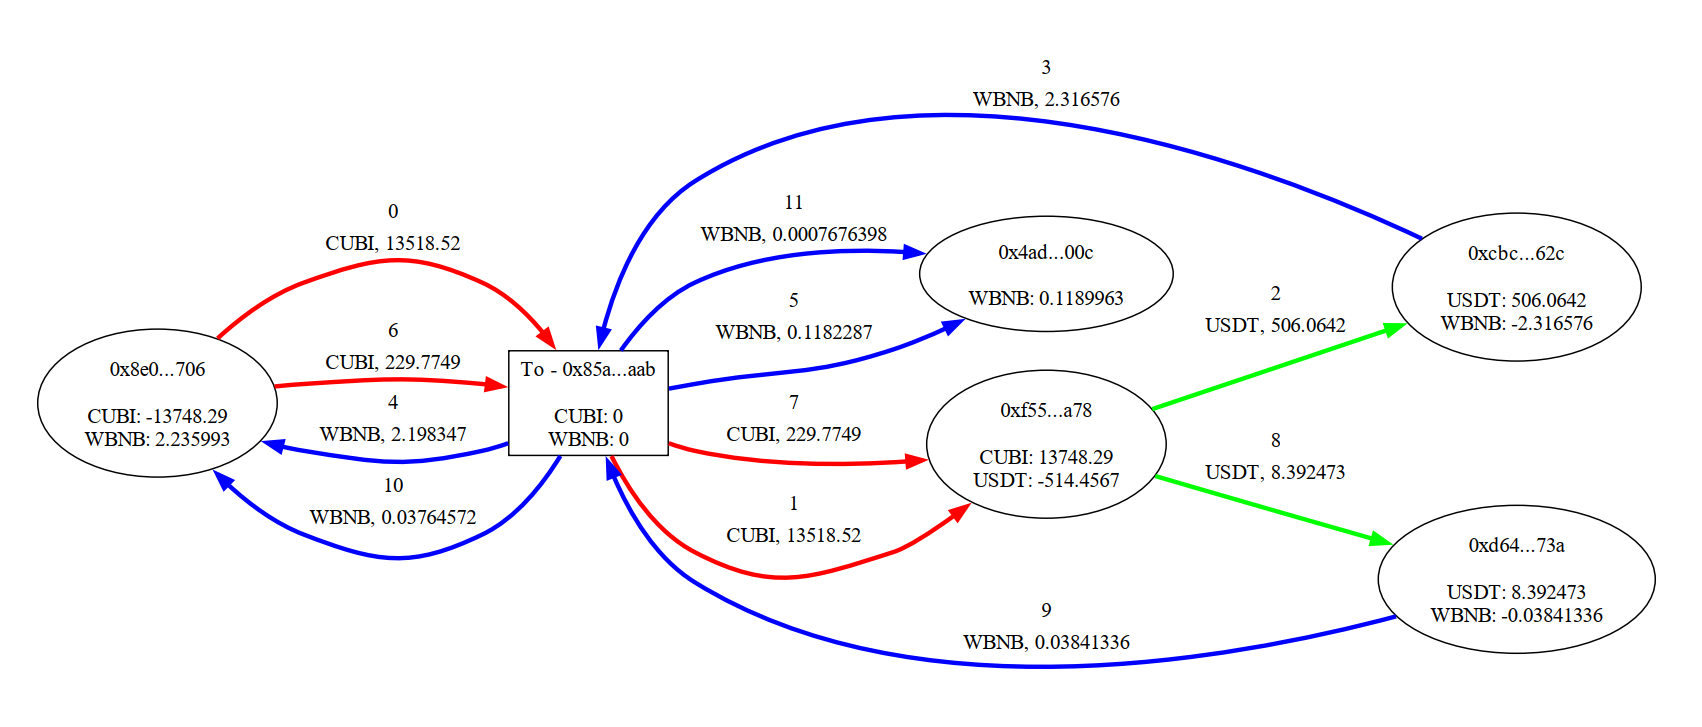
\includegraphics[scale=0.3]{img/arb1.png}
    \caption{Arbitražo vizualizacija: lėšų pervedimai ir galutinis pelnas – 0,11899 WBNB}
    \label{img:chess-minimax-2}
\end{figure} 

\ref{img:chess-minimax-2} pav. pateikta arbitražo vizualizacija kriptovaliutų atveju. Matome 12 pavedimų tarp skirtingų piniginių adresų (numeracija prasideda nuo 0). Šiuo atveju adresas 0x85a..aab yra pradinis kontrakto adresas, kuris buvo iškviestas tranzakcijoje. Iš viso tranzakcijoje dalyvauja 4 rinkos, kuriose galima konvertuoti valiutų poras:

\begin{itemize}
    \item 0x8eo..706 -- CUBI - WBNB
    \item 0xf55..a78 -- CUBI - USDT
    \item 0xcbc..62c -- USDT - WBNB
    \item 0xd64..73a -- USDT - WBNB
\end{itemize}

Adresas 0x4ad..00c šiuo atveju yra tik pelno piniginė, kurioje tranzakcijos pabaigoje atsiranda papildomi 0,11899 WBNB valiutos.

Kiekviename mazge taip pat pažymėtos valiutos ir jų kiekiai, nurodantys galutinį valiutos skirtumą po tranzakcijos. Pavyzdžiui, rinkoje 0x8eo..706 valiuta WBNB -> CUBI buvo konvertuota du kartus, kur iš viso į rinką įdėta 2,235993 WBNB, o išimta 13748,29 CUBI.

Tranzakciją galima suskirstyti į dvi dalis su pavedimais 0-5 ir 6-11. Pirmuosiuose penkiuose pavedimuose (0-4) atliekamas ratas: pradžioje trumpam pasiskolinama CUBI, tada ji iškeičiama į USDT, o po to -- į WBNB. Trečiuoju pavedimu gaunama daugiau valiutos, nei reikia skolai grąžinti ketvirtuoju pavedimu. Todėl perviršis lieka kaip pelnas, kuris penktuoju pavedimu persiunčiamas į pelno piniginę. Panašiai vyksta ir su pavedimais 6-11, tačiau antrojoje dalyje naudojama kita USDT-WBNB rinka, o apskritai keičiamų valiutos kiekių dydžiai yra mažesni.

\section{Likvidacijos}

Šiame skyriuje detaliai nagrinėjamas likvidavimo mechanizmas decentralizuotuose skolinimo protokoluose. Likvidacijos procesas yra esminė perviršinio užstato skolinimo platformų dalis, užtikrinanti jų stabilumą ir saugumą. Jo supratimas yra būtinas norint įvertinti, kaip automatizuoti algoritmai gali efektyviai išnaudoti šį mechanizmą pelno generavimui. Ši tema svarbi ne tik dėl praktinio aktualumo likvidatoriams, bet ir todėl, kad tai išskiria DeFi sistemų veikimą nuo tradicinių finansinių platformų. Skiriant daugiau dėmesio šiam procesui, galima tiksliau suformuluoti optimizavimo tikslus bei pagrįsti siūlomų strategijų svarbą.
% Koks yra sios analizes tikslas? Suprasti apie defi paskolu platformas ir kuo ju likvidavimo procesas issiskiria nuo tradiciniu finansu sistemu.

\subsection{Tradicinės paskolų platformos}
Paskolų platformos – tai sistemos, kuriose vartotojai gali skolintis ar skolinti pinigus kitiems vartotojams. Tradicinėse bankinėse sistemose bankas veikia kaip tarpininkas tarp skolintojo ir skolininko. Panašiai veikia ir kredito unijos, kuriose nariai vieni kitiems suteikia paskolas per bendrą fondą.

\subsubsection{Veiklos principas}
\begin{itemize}
    \item \textbf{Skolintojai}: asmenys ar įmonės, turintys perteklinių lėšų, kurias jie norėtų investuoti, kad gautų grąžą kaip palūkanas.
    \item \textbf{Skolininkai}: asmenys ar įmonės, kuriems reikia lėšų įvairiems tikslams – pradėti verslą, finansuoti projektą, pirkti prekę ir pan.
\end{itemize}

Skolintojai įneša savo lėšas į platformą, o skolininkai pateikia prašymus dėl paskolų. Platforma tada suderina šiuos du suinteresuotus šalių poreikius. Priklausomai nuo platformos ir paskolos tipo, gali būti reikalaujama, kad skolininkai užstatytų tam tikrą turto dalį kaip garantiją.

\subsubsection{Likvidacijos tradicinėse sistemose}
Tradicinėse finansų sistemose likvidacija vyksta tuomet, kai skolininkas nesugeba įvykdyti savo įsipareigojimų grąžinti paskolą. Tokiu atveju kredito įstaiga (bankas ar kredito unija) gali pradėti priverstinį skolų išieškojimo procesą, kuris dažnai apima užstato realizavimą.

Procesas dažnai prasideda nuo skolininko įspėjimo apie neįvykdytą mokėjimą. Jeigu situacija nesikeičia, kreditorius gali inicijuoti teisinį procesą: kreiptis į antstolius arba teismą dėl turto arešto ir pardavimo. Užstatas, pavyzdžiui, nekilnojamasis turtas ar transporto priemonė, įvertinamas ir parduodamas aukcione arba per kitus kanalus.

Gautos lėšos naudojamos skolos padengimui. Jeigu užstato realizavimo suma viršija skolos vertę, likutis grąžinamas skolininkui. Priešingu atveju, jei skolos likutis išlieka, skolininkas lieka skolingas likusią sumą. Procesas yra ilgesnis nei automatizuotose sistemose, tačiau suteikia galimybę ginčams spręsti ir apsaugoti abi puses teisinėmis priemonėmis.

\subsection{Kriptovaliutų paskolų platformos}
Šiuolaikinėse paskolų platformose populiarėja kriptovaliutų paskolų modelis, kuriame operacijos atliekamos naudojant kriptovaliutas arba kitą kriptoturtą kaip užstatą. Skolinimo ir grąžinimo procesai šiose platformose vykdomi naudojant išmaniuosius kontraktus. Tokios platformos priklauso decentralizuotų finansų sistemai – tai finansinių paslaugų ekosistema, veikianti be tarpininkų, pagrįsta blokų grandinės technologija ir automatizuota išmaniųjų kontraktų pagalba.

Viena iš svarbiausių šių platformų savybių yra tai, kad skolininkai privalo pateikti užstatą, kuris viršija paimtos paskolos vertę. Kriptovaliutų pasaulyje tokia perviršinio užstato sistema yra būtina, nes leidimas skolintis daugiau nei pateikto užstato vertė atvertų kelią reikšmingam išnaudojimui. Jei būtų galima pateikti mažai užstato ir gauti didelę paskolą, tai sukeltų didelę riziką platformai, nes skolininkai galėtų nesąžiningai išnaudoti šią galimybę, o skolintojai patirtų didžiulius nuostolius. Todėl perviršinio užstato reikalavimas yra esminis saugumo mechanizmas, užtikrinantis stabilumą ir patikimumą šiose finansinėse sistemose. \cite{whatisdefiliquidation}

Dar viena kriptovaliutų paskolų platformų ypatybė -- tai valiutų vertės nustatymo procesas, kuris yra atliekamas naudojant orakulus. Orakulai yra išoriniai informacijos tiekėjai, kurie pateikia duomenų srautą naudojantis išmaniaisiais kontraktais. Šie kontraktai yra periodiškai atnaujinami per privilegijuotas \textit{blockchain} tranzakcijas. Šios tranzakcijos nustato tam tikros valiutos vertę, užtikrindamos sklandų ir patikimą platformos veikimą.

\subsubsection{Kodėl žmonės skolinasi per kriptovaliutų paskolų platformas?}

\begin{enumerate}
    \item \textbf{Kapitalo prieinamumas neparduodant turto}: skolinantis per kriptovaliutų platformas, galima gauti lėšų neparduodant turimų kriptovaliutų, taip išvengiant galimų mokesčių ir toliau dalyvaujant rinkos augime \cite{kriptovaliutosio}.
    \item \textbf{Greitas ir paprastas procesas}: kriptovaliutų paskolos dažnai suteikiamos greičiau ir su mažiau biurokratijos nei tradicinės bankų paskolos, nes nereikalaujama kredito istorijos patikrinimo \cite{targettrend}.
    \item \textbf{Trumpasis pardavimas}: dar angliškai vadinamas \textit{shorting}. Kriptovaliutų skolinimo platformos leidžia naudotojams skolintis kriptovaliutas, kurias jie vėliau parduoda dabartine rinkos kaina tikėdamiesi kainų kritimo ateityje. Kainai nukritus yra nuperkamas tas pats kiekis valiutos, kiek buvo pasiskolinta, ir iš karto gražinama skola. Šis metodas leidžia investuotojams uždirbti iš rinkos kainų svyravimų net ir krintant kainoms. Pavyzdžiui, investuotojas gali užstatyti savo ETH, pasiskolinti BTC, parduoti BTC už \$30\,000, tariant, kad einamuoju metu yra tokia kaina, ir vėliau nusipirkti už \$25\,000, tariant, kad po kažkiek laiko kaina nukrito, grąžindamas skolą ir pasilikdamas \$5\,000 pelno.
    \cite{shortinimas}.
\end{enumerate}

\subsubsection{DeFi likvidacijų palyginimas su tradicinę finansų sistemą}
DeFi likvidacijos procesas skiriasi nuo tradicinio likvidavimo keliais esminiais aspektais, kurie yra svarbūs norint suprasti, kodėl šiose sistemose leidžiama įtraukti daugiau dalyvių – trečiąsias šalis, atliekančias likvidaciją \cite{whatisdefiliquidation}:

\begin{itemize}
    \item \textbf{Automatizavimas:} DeFi likvidacijos paprastai yra automatizuotos naudojant išmaniuosius kontraktus, todėl nereikia žmogaus įsikišimo. Tradicinėse finansų sistemose maržos reikalavimas dažnai reikalauja skolininko ar tarpininko rankinio veiksmo.
    
    \item \textbf{Skaidrumas:} DeFi likvidacija yra visiškai skaidri – visos tranzakcijos vyksta viešoje blokų grandinėje. Tradicinėse finansų sistemose likvidacijos detalės gali būti sunkiau prieinamos ar nematomos plačiajai visuomenei.
    
    \item \textbf{Decentralizacija:} DeFi veikia be tarpininkų – kriptovaliutų likvidacijos vykdomos tiesiogiai per kodo logiką. Tradicinėse finansų sistemose likvidacijas valdo brokeriai arba finansinės institucijos.
\end{itemize}

Kai skolininko užstato vertė krinta žemiau likvidavimo ribos, pagal protokolą bet kam leidžiama atlikti likvidaciją. Per likvidacijos procesą užstatas yra parduodamas, dažnai su tam tikra nuolaida, mainais į valiutą, kurią skolininkas pasiskolino. \cite{venussavokosbendras}

\subsubsection{Protokolai}

Yra daugybė paskolų protokolų, veikiančių įvairiuose \textit{blockchain} tinkluose, kurie suteikia vartotojams galimybę skolintis ir skolinti decentralizuotai. \ref{tab:sample_table} lentelėje pateikiami keli populiariausi šių protokolų pavyzdžiai. 

\begin{itemize}
  \item \textbf{Blokų grandinės} – išvardijami \textit{blockchain} tinklai, kuriuose veikia atitinkamas protokolas. Paskolų mechanizmas tarp tinklų gali skirtis dėl tinklo subtilybių, tačiau pagrindiniai procesai išlieka tokie pat tam pačiam protokolui.
  \item \textbf{Bendra užrakinta vertė} – angl. \textit{Total Value Locked}, atspindi platformos bendrą turto vertę įdėtą naudotojų. Tai svarbus rodiklis, leidžiantis įvertinti protokolo populiarumą ir pasitikėjimą. Paskolų platformų kontekste, ši vertė nurodo bendrą užstato sumą, iš kurios kaupiamos palūkanos už paskolintą turtą.
  \end{itemize}
  
Iš lentelės matome, kad Aave yra vienas iš populiariausių ir labiausiai paplitusių paskolų protokolų, veikiantis daugybėje \textit{blockchain} tinklų ir turintis didžiausią bendrą užrakintą vertę – \$22,112 milijardų. Šis protokolas išsiskiria savo plačia integracija ir stipriu vartotojų pasitikėjimu.

\begin{table}[H]
  \centering
  \caption{Paskolų protokolų sąrašas \cite{LikvidacijuProtokolai}}
  \begin{tabular}{|l|p{7cm}|p{5cm}|}
  \hline
  \textbf{Pavadinimas} & \textbf{Blokų grandinės} & \textbf{Bendra užrakinta vertė} \\ \hline
  Aave                      & Ethereum, Base, Polygon, Hyperliquid L1, World Chain, OP Mainnet, Corn, Arbitrum, Fraxtal, Sonic, Plume Mainnet, Ink, Hemi, Mode, Basecamp, Unichain, Scroll, Flame & \$24,867B \\ \hline
  JustLend                  & Tron                                                & \$5,168B  \\ \hline
  Morpho                    & Ethereum, Base                                      & \$3,526B  \\ \hline
  SparkLend                 & Ethereum, Gnosis                                    & \$3,054B  \\ \hline
  Compound Finance          & Ethereum, Arbitrum, Base, Polygon, OP Mainnet, Mantle, Unichain, Ronin, Scroll & \$2,626B  \\ \hline
  Kamino Lend               & Solana                                              & \$2,186B  \\ \hline
  Venus                     & BSC, ZKsync Era, Arbitrum, opBNB, Ethereum, Unichain, Base, OP Mainnet          & \$1,692B  \\ \hline
  Maple                     & Ethereum, Solana          & \$1,082B  \\ \hline
  Fluid Lending             & Ethereum, Arbitrum, Polygon, Base                            & \$989,61M \\ \hline
  Euler                     & Ethereum, Avalanche, Sonic, BSC, Base, Swellchain, BOB, Berachain, Unichain          & \$937,26M  \\ \hline
  Suilend                   & Sui                                                 & \$682,96M \\ \hline
  NAVI Lending              & Sui                                                 & \$542,57M \\ \hline
  Lista Lending                     & BSC          & \$531,02M  \\ \hline
  Avalon Labs               & Ethereum, BSC, Sonic, Berachain, Mantle, Bitlayer, Taiko, BOB, Merlin, DuckChain, ZetaChain, IoTeX, Kaia, Arbitrum, Base, CORE, Corn, BSquared, Mode, Sei, Scroll, Zircuit & \$459,62M  \\ \hline
  Aries Markets                     & Aptos          & \$414,59M  \\ \hline
  \end{tabular}
  \label{tab:sample_table}
\end{table}

\subsubsection{Venus platforma}
Šiame darbe toliau yra analizuojamas \textit{Venus} protokolas ir jo istorinės likvidacijos. Nors ši platforma nėra didžiausia, jos likvidavimo mechanizmai yra panašūs į daugelio kitų kriptovaliutų paskolų platformų. Tai bus detaliau parodyta skyriuje \ref{sec:venus_mechanizmas}

\textit{Venus} protokolas pasirinktas dėl autoriaus asmeninio susipažinimo su jo veikimu ir ilgametės patirties pagrindiniame jo \textit{blockchain} tinkle – \textit{Binance Smart Chain}.

\subsubsection{Arbitražo potencialas}
Iš esmės, likvidaciją galima laikyti tam tikra rinka, suteikiančia galimybę konvertuoti vieną valiutą į kitą. Likvidacija paprastai yra pelninga likviduotojams, nes pasiskolinta valiuta yra iškeičiama į užstatą, kurio vertė dažnai viršija grąžintos paskolos sumą – taip likvidatoriams sukuriama finansinė paskata veikti. Ši procedūra yra nepalanki skolininkui, nes jis priverstinai praranda dalį arba visą savo užstatą. Skolintojams likvidacija naudinga tuo, kad užtikrina paskolos grąžinimą net ir tuomet, kai skolininkas pats to padaryti nesugeba. Todėl likvidacijos procesas yra naudingas likviduotojams ir skolintojams, tačiau nuostolinga skolininkui.

Jeigu valiuta, kuria reikia grąžinti skolą, yra nestabili iš likvidatoriaus perspektyvos, galima konvertuoti turima kapitalą iš stabilios valiutos į skolinamąją valiutą. Panašiai, užstato valiutą galima konvertuoti į stabilų piniginį vienetą per tam tikras valiutų keitimo operacijas kitose rinkose. Tokiu atveju, arbitražo sistema tampa itin vertinga, nes ji gali automatizuoti valiutos konversijos procesą ir rasti efektyviausią būdą konvertuoti iš valiutos A į valiutą B, tuo pačiu užtikrinant, kad likvidatorius gaus maksimalų pelną.

Taigi, jeigu turime algoritmą, kuris sugeba aptikti arbitražo galimybes iš tam tikros rinkų aibės, šią aibę galima papildyti likvidacijos rinkomis, leidžiant likvidatoriams bandyti pasipelnyti iš likvidacijų su minimalia ar net be rizikos. Tačiau likvidatoriai gali susidurti su rizikomis -- pavyzdžiui, būti aplenktiems kitų likvidatorių arba mokėti mokesčius už bandymus atlikti likvidaciją be sėkmingo likvidavimo dėl klaidos ar būsenos pasikeitimo, kuri nebeleistų atlikti valiutų konvertavimo. Šios rizikos yra aktualios ir paprastesniems arbitražo scenarijams tarp rinkų.

\section{Venus protokolo likvidavimo mechanizmas}
\label{sec:venus_mechanizmas}

Šiame skyriuje siekiama išsamiai išanalizuoti \textit{Venus} protokolo likvidavimo mechanizmą \cite{venusprotocolcode}, suprasti jo veikimo principus bei išskirti pagrindinius parametrus, lemiančius likvidacijos eigą. Nors pasirinktas konkretus protokolas, analizė nėra skirta tik jam – šiuo tyrimu taip pat siekiama įvertinti, kiek \textit{Venus} modelis yra atstovaujantis platesnei kriptovaliutų paskolų platformų ekosistemai. Lyginant su kitais protokolais, bus siekiama pagrįsti, kad tolimesni šiame darbe siūlomi algoritmai gali būti taikomi ir kitose panašaus tipo decentralizuotose skolinimo sistemose.

\subsection{Sąvokos}
Šiame skyriuje pateikiamos pagrindinės su likvidacija susijusios sąvokos. \cite{venussavokosbendras, aavelikvidacijos}
\begin{itemize}
  \item \textbf{Pozicija (angl. \textit{position})}: rinkinys kelių užstatų ir paskolų, suskirstytų pagal valiutą, kuriuos valdo vienas naudotojas.
  \item \textbf{Užstato koeficientas / Paskolos ir užstato santykis (angl. \textit{collateral factor, CF} / \textit{loan to value, LTV})}: procentinė dalis, kuria užstato vertė įtraukiama į skolinimosi pajėgumą. Kiekviena valiuta turi atskirą vertę (paprastai nuo 60\% iki 90\%).
  \item \textbf{Skolinimosi pajėgumas (angl. \textit{borrowing capacity, BC})}: apibrėžia bendrą vertę, kurią skolininkas gali pasiskolinti, atsižvelgiant į jo užstato sumą.
    \begin{equation}
        BC = \sum_{i} \bigl(\text{Užstato vertė}_{i} \times CF_{i}\bigr), \quad \text{kur } i \text{ žymi } i\text{-ąją valiutą pozicijoje}
        \label{eq:borrowing_capacity}
    \end{equation}
  \item \textbf{Sveikumo koeficientas (angl. \textit{health factor, HF})}: matuoja pozicijos būklę, apibrėžiamą kaip skolinimosi pajėgumo ir esamų skolų santykį. Jeigu sveikumo koeficientas mažesnis negu 1, skolininkas tampa likviduojamas.
    \begin{equation}
        HF = \frac{BC}{\sum_{i} \text{Skolos vertė}_{i}}
        \label{eq:health_factor}
    \end{equation}
  \item \textbf{Likvidavimo slenkstis (angl. \textit{liquidation threshold})}: riba, nuo kurios skolininkas tampa likviduojamas.
  \item \textbf{Uždarymo riba (angl. \textit{close factor})}: maksimali skolos dalis, kuri leidžiama būti grąžinta vienos likvidacijos metu. Vertė yra bendra visam protokolui, mūsų atveju 50\%.
  \item \textbf{Likvidacijos paskata}: priedas arba nuolaida, kurią likvidatorius gali gauti, likviduodamas užstatą.
  Šis skirtumas skatina likvidatorius veikti nedelsiant, kai paskola peržengia likvidavimo slenkstį. \textit{Venus} atveju tai yra 10\% gražinamos valiutos vertės.
\end{itemize}

\subsection{Likvidacijos ypatumai}
\label{sec:likivdacijos_ypatumai}

Skolininkui tapus likviduojamu, yra daugybė pasirinkimų, kaip vykdyti jo pozicijos likvidavimą. Likvidavimo proceso metu būtina pasirinkti konkrečią užstato ir paskolos valiutų porą, kurioje paskolos valiuta yra grąžinama, o užstato valiuta paimama iš skolininko. Taip pat, nustatomas grąžintinos sumos dydis. Svarbu pabrėžti, jog atlikus nedidelę likvidaciją, skolininkas gali išlikti likviduojamas, tai reiškia, kad likvidavimo procesas gali būti vykdomas kelis kartus.

Svarbu pažymėti, kad likvidavimo metu protokolas leidžia likviduoti didesnį valiutos kiekį, nei būtina skolininko pozicijai subalansuoti. Tarkime:
\begin{itemize}
  \item skolininkas yra pateikęs \$2\,000 vertės BTC (bitkoino) valiutą kaip užstatą;
  \item BTC valiutos užstato koeficientas (\textit{CF}) yra 80\%;
  \item skolininkas yra pasiskolinęs 1\,650 USDT valiutos, kuri atitinka JAV dolerį.
\end{itemize}

Toliau \ref{tab:likvidacijos_pav} lentelėje matyti, kaip šios vertės kinta po skirtingo dydžio likvidacijų.
Pirmuoju variantu grąžinama \$417, po kurios skolininko sveikumo koeficientas pakyla virš 1, todėl
skolininko pozicija nustoja būti likviduojama.
Antruoju variantu grąžinama maksimali suma, kiek leidžiama, kai uždarymo riba lygi 50\%.
Šiuo atveju pozicija taip pat tampa „sveika“, tačiau skolininkas patiria didesnį nuostolį, o likvidatorius – didesnį pelną.

\begin{table}[h!]
  \centering
  \caption{Pavyzdinė užstato, skolos ir sveikumo koeficiento kaita po likvidacijos}
  \begin{tabular}{lccccc}
  \hline
  \textbf{Būsena} 
  & \textbf{Užstato vertė}
  & \textbf{Skolos vertė}
  & \textbf{BC}
  & \textbf{HF}
  & \makecell{\textbf{Pelnas likvidatoriui /}\\ \textbf{nuostolis skolininkui}} \\ 
  \hline
  Pradinė                
  & 2000      
  & 1650      
  & 1600      
  & 0,97    
  & --         \\
  
  Po \$417 likvidacijos  
  & 1541,3    
  & 1233      
  & 1233,04   
  & 1,00003   
  & 41,7       \\
  
  Po \$825 likvidacijos  
  & 1092,5    
  & 825       
  & 874       
  & 1,06      
  & 82,5       \\
  \hline
  \end{tabular}
  \label{tab:likvidacijos_pav}
  \end{table}

Likvidatoriams yra naudinga grąžinti kuo didesnę skolą už skolininką, nes už grąžintą paskolos valiutą atlyginama tokios pačios vertės užstatu, be to, papildomai suteikiama 10\% užstato kaip paskata. Likvidatorių procesą riboja du pagrindiniai dalykai: skolininko užstato dydis ir uždarymo riba.

Jeigu likvidatorius siekia vykdyti arbitražą, jis taip pat turi įvertinti kainos pokytį, kuris įvyks keičiant valiutas kitose rinkose. Dideli valiutų keitimai lemia didesnius kainos svyravimus nepalankia kryptimi. Todėl likvidatoriaus veiksmus netiesiogiai riboja ir kitų rinkų likvidumas. Jei valiutos likvidumas yra mažas, orakulo nurodyta kaina gali reikšmingai skirtis nuo realios rinkos kainos. Tokiais atvejais gali susidaryti situacija, kai net ir turėdamas galimybę atlikti didelės vertės (milijonų dolerių) likvidaciją, likvidatorius jos nevykdys, nes užstatas būtų realizuojamas gerokai žemesne kaina nei ta, kurią tuo metu rodo orakulas. 

\subsection{Panašumai su kitais protokolais}
\label{sec:panasumai_su_kitais_protokolais}

Nors šiame darbe pagrindinis dėmesys skiriamas \textit{Venus} protokolo likvidavimo mechanizmo analizei, būtina pažymėti, kad šis mechanizmas yra itin panašus į kitų reikšmingų decentralizuotų skolinimo protokolų, tokių kaip \textit{Aave} ir \textit{Compound}, veikimą. Dėl šios priežasties \textit{Venus} galima laikyti reprezentatyviu DeFi skolinimo sistemų atveju, o šiame darbe siūlomos strategijos gali būti aktualios ir taikomos kitų protokolų kontekste.

\textit{Venus} buvo sukurtas remiantis \textit{Compound} ir \textit{MakerDAO} protokolų pagrindu, perėmus jų funkcionalumą ir apjungus jį į vieną bendrą sistemą \cite{whatisvenus}. Nors \textit{MakerDAO} daugiausiai orientuojasi į stabilios valiutos (DAI) išleidimą, \textit{Compound} pasižymi išplėtota skolinimo infrastruktūra, kurią \textit{Venus} ir perėmė.

\textit{Compound} protokolas turi tris pagrindines versijas: V1, V2 ir V3. Versija V2, pristatyta 2019 m. gegužę \cite{compound2launch}, įvedė reikšmingus architektūrinius pokyčius, tarp jų – atskirus rinkos kontraktus kiekvienai valiutai bei cToken mechanizmą, leidžiantį naudotojams uždirbti palūkanas bei naudoti savo turtą kaip užstatą. Šios V2 versijos savybės yra esminės \textit{Venus} protokolo struktūrai. Be to, remiantis DeFiLlama duomenimis, \textit{Venus} oficialiai priskiriamas \textit{Compound V2} forkų grupei, o tai papildomai patvirtina architektūrinį paveldimumą \cite{venuscompoundfork}.

% V3 versija (dar vadinama Comet) ženkliai skiriasi nuo ankstesnių ir nuo Venus protokolo.

\paragraph{Struktūriniai panašumai} Toliau apžvelgiami pagrindiniai veikimo aspektai, kuriuose \textit{Venus}, \textit{Compound} (V2) ir \textit{Aave} pasižymi esminiais panašumais:

\begin{itemize}
    \item \textbf{Pozicijų struktūra.} Visuose minėtuose protokoluose naudotojo pozicija sudaryta iš paskolų ir užstatų, suskirstytų pagal konkrečias valiutas. Bendras pozicijos sveikumo koeficientas skaičiuojamas pagal visų paskolos ir užstato komponentų santykį, atsižvelgiant į kiekvienos valiutos užstato koeficientą. Tokia formulė taikoma tiek \textit{Aave}, tiek \textit{Compound}, tiek \textit{Venus} sistemose \cite{aave-risks, compound-positionstructure}.

    \item \textbf{Uždarymo riba.} Visi trys protokolai riboja vienos likvidacijos metu grąžinamos paskolos dalį. \textit{Venus} ir \textit{Compound} V2 naudoja 50\% fiksuotą ribą \cite{compound-closefactor}, o \textit{Aave} leidžia šią reikšmę konfigūruoti intervale nuo 50\% iki 100\%, priklausomai nuo paskolos rizikos parametrų \cite{aave-liquidation}.

    \item \textbf{Likvidacijos poromis.} Visuose aptariamuose protokoluose likvidavimas vykdomas poromis – t. y., likvidatorius pasirenka konkrečią skolos valiutą, kurią grąžina, ir užstato valiutą, kurią atsiima. Likvidacija nevykdoma visos pozicijos mastu, bet yra realizuojama per konkrečias skolos–užstato valiutų poras \cite{compound-liquidation, aave-liquidation}.
\end{itemize}

\paragraph{Skirtumai} Nepaisant reikšmingų panašumų, tam tikri struktūriniai skirtumai tarp šių protokolų visgi egzistuoja:

\begin{itemize}
    \item \textbf{Likvidacijos paskata.} \textit{Venus} protokole likvidacijos paskata (angl. \textit{liquidation incentive}) yra fiksuota visoms valiutoms ir siekia 10\%. Tuo tarpu \textit{Aave} ir \textit{Compound} leidžia šią paskatą konfigūruoti atskirai kiekvienai užstato valiutai, kas suteikia daugiau lankstumo rizikos valdymo požiūriu \cite{compound-incentive, aave-liquidation}.

    \item \textbf{Skirtingi užstato koeficientai.} \textit{Aave} protokole užstato koeficientai skolinimuisi ir likvidacijai gali skirtis – vadinamasis \textit{liquidation threshold} dažnai būna didesnis už skolinimosi limitą. Toks sprendimas leidžia apsaugoti protokolą ir naudotojus, sukuriant papildomą „apsauginį buferį“ nuo nedidelių kainos svyravimų.
\end{itemize}

\paragraph{Apibendrinimas}

Atsižvelgiant į šiuos aspektus, galima teigti, kad \textit{Venus} protokolo architektūra yra labai artima \textit{Compound V2} modelio įgyvendinimui, tuo pačiu perimdama ir tam tikrus \textit{Aave} veikimo principus. Dėl šios priežasties \textit{Venus} gali būti laikomas reprezentatyviu decentralizuotų paskolų platformų pavyzdžiu, o šiame darbe taikomos ir analizuojamos strategijos – aktualios ir kitiems populiariems protokolams, taikantiems analogiškus likvidavimo principus.

\section{Skirtingos likvidacijų strategijos}
\label{sec:liq_strategijos}

Šiame skyriuje pateikiami skirtingi likvidavimo metodai. Pirmiausia aprašomi paprasti, intuityvūs metodai, kuriuos nesudėtinga sugalvoti. Vėliau apžvelgiama esama literatūra, siūlanti efektyvius likvidavimo būdus. Taip pat pristatomi autoriaus pasiūlyti patobulinimai, atsižvelgiant į \textit{Venus} protokolo ypatumus. Galiausiai analizuojamos strategijos, kurios taikomos likviduojant keletą skirtingų valiutų porų.

\subsection{Naivus algoritmas}
\label{sec:largest_borrow}

Paprasta likvidavimo algoritmo idėja gali būti tokia: turint likviduojamo skolininko poziciją, pasirenkama paskolos valiuta, kuriai skolininkas turi didžiausią įsipareigojimą, ir užstato valiuta, kurios vertė skolininko pozicijoje yra didžiausia. Tuomet stengiamasi grąžinti tiek, kiek leidžia uždarymo riba (paprastai – pusę pasiskolintos valiutos vertės), arba tiek, kad būtų išnaudotas visas skolininko užstatas pasirinkta valiuta. Kadangi praktikoje dažniau pasiekiama uždarymo riba, o ne užstato apribojimas, šiai strategijai suteikiame pavadinimą – \textit{didžiausia skola}.

Ši strategija literatūroje dar kartais vadinama \textit{iki uždarymo ribos} (angl. \textit{up to close factor}) \cite{Emp}. Šiame darbe abu terminai vartojami skirtinguose kontekstuose: kai galime laisvai pasirinkti skolos ir užstato valiutas, strategija vadinama \textit{didžiausia skola}, o kai valiutų pora jau yra fiksuota, vartojamas pavadinimas \textit{iki uždarymo ribos}.

Svarbu pažymėti, kad skolininko užstato vertė yra ribojama išgryninimo galimybėmis – paskolų platformose likvidatorius užstatą gauna apgaubta forma, kurią reikia papildomai konvertuoti į grynąją valiutą. Gali kilti situacijų, kai grynoji užstato forma tuo metu yra nepasiekiama, nes visa valiuta yra paskolinta kitiems skolininkams. Dėl to ne visada įmanoma iš karto atsiimti visą užstato vertę. Toliau šiame darbe, kalbant apie skolininko užstato vertę, bus daroma prielaida, kad kalbama apie skolininko užstato dalį, kurią galima tuo metu išsigryninti.

\ref{tab:naivus_pav} lentelėje pateikti trys scenarijai su skolininko pozicijomis, kuriose, tarkime, visi skolininkai yra likviduojami:
\begin{enumerate}
    \item \textbf{Pirmas scenarijus:} renkamės ETH valiutą kaip grąžinamą, nes taip galima grąžinti didžiausią vertę (\$500). Grąžinant šią sumą iš skolininko užstato galima paimti \$550 vertės turto. Kadangi BNB yra tik \$500, to nepakanka, todėl renkamės valiutą su didžiausiu užstatu – BTC.
    
    \item \textbf{Antras scenarijus:} renkamės USDT kaip grąžinamą valiutą, o ETH – kaip užstatą, nes jo vertė didžiausia. Tiesa, šiuo atveju pakaktų ir AVAX užstato, nes grąžindami didžiausią leistiną sumą (\$1\,000) galime paimti \$1\,100 vertės turto. Jei AVAX valiutą būtų lengviau parduoti rinkoje, likvidatorius galėtų rinktis ją.

    \item \textbf{Trečias scenarijus:} iš kelių užstato variantų renkamės ETH, nes jo vertė didžiausia, o grąžinama valiuta bus USDC (taip pat dėl didžiausios sumos). Iš tikrųjų bet kuri grąžinama valiuta leistų padengti tokią sumą, jog būtų galima paimti visą ETH užstatą, nes tereikia grąžinti $\frac{\$500}{1,1} \approx \$454,54$ skolos.
\end{enumerate}

\begin{table}[h!]
  \centering
  \caption{Pavyzdiniai skolininko pozicijų duomenys su įvairiomis skolomis ir užstatais}
  \begin{tabular}{lcc}
  \hline
  \textbf{Pozicija} 
   & \textbf{Skolos} 
   & \textbf{Užstatai} \\
  \hline
  1 & 
  \begin{tabular}[c]{@{}l@{}}ETH: \$1000 \\ DAI: \$500 \\ USDC: \$300\end{tabular} 
   & \begin{tabular}[c]{@{}l@{}}BTC: \$2000 \\ BNB: \$500\end{tabular} \\
  \hline
  2 &
  \begin{tabular}[c]{@{}l@{}}USDT: \$2000 \\ DAI: \$400\end{tabular}
   & \begin{tabular}[c]{@{}l@{}}ETH: \$3000 \\ AVAX: \$1500\end{tabular} \\
  \hline
  3 &
  \begin{tabular}[c]{@{}l@{}}USDC: \$1500 \\ WBTC: \$800\end{tabular}
   & \begin{tabular}[c]{@{}l@{}}ETH: \$500 \\ SOL: \$400 \\ AVAX: \$400 \\ BNB: \$400\end{tabular} \\
  \hline
  \end{tabular}
  \label{tab:naivus_pav}
  \end{table}

\subsection{Esami tyrimai}
\label{sec:esami_tyrimai}

Šioje srityje jau egzistuoja mokslinių darbų, siūlančių algoritmus likvidavimo problemoms spręsti. Pavyzdžiui, \cite{Emp} pristato algoritmą \textit{Optimal Fixed Spread Liquidation Strategy}, kuris padalina likvidavimo procesą į dvi mažesnes likvidacijas, kurias kartu sudėjus, leidžia likviduoti didesnį kiekį nei būtų galima padaryti tik su vienu dideliu likvidacijos iškvietimu. Pirmoji likvidacija yra maksimaliai didelė, taip, kad po jos skolininkas vis dar lieka likviduojamas, reiškia, jog sveikumo koeficientas (\textit{HF}) yra kiek įmanoma didesnis, bet mažesnis nei 1. Antroji likvidacija užbaigia procesą, likviduojant maksimalų kiekį, kurį leidžia protokolo taisyklės, vienu likvidacijos iškvietimu, kas paprastai reiškia 50\% likusios paskolos dydžio. Ši strategija veikia tik tada, kai yra iš anksto nurodyta skolos ir užstato valiutų pora – ji pati nenusako, kokią porą pasirinkti, o siekia maksimaliai padidinti likvidacijos dydį konkrečiai pateiktoje poroje.

\textit{Venus} protokolui \textit{Optimal Fixed Spread Liquidation Strategy} algoritmas nėra tinkamas, nes grąžinant pagrindinio tinklo valiutą (šiuo atveju BNB) pasikeičia kursas, pagal kurį apgaubtas užstatas konvertuojamas į pagrindinę valiutą. Kurso perskaičiavimas įvyksta prieš pat nustatant skolininko pozicijos sveikumo koeficientą ($HF$). Dėl to didelės grąžinamos sumos gali reikšmingai paveikti skolininko likvidumo būklę, sumažindamos likvidacijos ribą arba netgi visiškai sustabdydamos likvidavimo procesą. Pagrindinė problema su algoritmu yra ta, kad pirmoji likvidacija, nors formaliai palieka skolininką likviduojamą, tam tikrais atvejais leidžia likviduoti tik labai mažas sumas antrojoje likvidacijoje.

Tam tikrais atvejais, kai skolininko įsiskolinimas yra itin didelis, gali būti vykdomos daugiau nei dvi likvidacijos, kiekvieną kartą likviduojant iki uždarymo ribos. Tačiau minėtas algoritmas apsiriboja tik dviem likvidacijų iškvietimais.

\subsection{Pasiūlyta \textit{Optimal Fixed Spread Liquidation Strategy} modifikacija}

Siūlome koreguoti \textit{Optimal Fixed Spread Liquidation Strategy}. Visų pirma, neapsiribosime dviem likvidacijos iškvietimais. Proceso pradžioje sukame ciklą, kurio metu kiekvieno iteracijos pradžioje apskaičiuojame $\text{B}_{\text{uždarymo}}$ ir $\text{B}_{\text{užstato}}$, kur:

\begin{itemize}
\item $\text{B}_{\text{uždarymo}}$ – maksimalus grąžinamos valiutos kiekis, leidžiamas likviduoti vienu kartu pagal uždarymo ribos taisyklę.
\item $\text{B}_{\text{užstato}}$ – grąžinamos valiutos kiekis, reikalingas visiškai atsiimti skolininko užstatą pasirinkta valiuta.
\end{itemize}

Jei $\text{B}_{\text{užstato}} \leq \text{B}_{\text{uždarymo}}$, vadinasi, kita likvidacija bus paskutinė, ir grąžiname $\text{B}_{\text{užstato}}$ pasiskolintos valiutos kiekį. Šios logikos privalumas yra tas, kad jei pirmosios likvidacijos dydis yra ribojamas užstato trūkumo, procesas gali būti baigtas per vieną likvidaciją. Tai leidžia maksimaliai efektyviai išnaudoti galimybes, sumažinant nereikalingų skaičiavimų, už kuriuos reikia sumokėti pagrindine valiuta, kiekį.

Kitu atveju ($\text{B}_{\text{užstato}} > \text{B}_{\text{uždarymo}}$), ieškome didžiausio $\text{B}_{i}$ tokio, kad po likvidacijos vis dar būtų galima likviduoti bent $\text{B}_{\text{užstato}} - \text{B}_{i}$. Jei rastas $\text{B}_{i} > 0$, atlikus likvidaciją grįžtame į ciklo pradžią. Jei $\text{B}_{i} = 0$, reiškia, bet koks likvidacijos dydis pavers skolininką nelikviduojamu. Tokiu atveju likviduojama $\text{B}_{\text{uždarymo}}$ ir į ciklo pradžią nebegrįžtama.

Galima įsivaizduoti, kad \ref{sec:esami_tyrimai} skyriuje aprašytas algoritmas taip pat ieško didžiausio $\text{B}_{i}$ pirmajai likvidacijai, užtikrinančio, jog po jos skolininkas išliks likviduojamas. Tačiau mūsų algoritmas reikalauja ne tik, kad skolininkas išliktų likviduojamas, bet ir kad būtų galima likviduoti reikšmingą kiekį valiutos. Šis papildomas reikalavimas yra ypač aktualus tais atvejais, kai grąžinama valiuta yra pagrindinė blokų grandinės valiuta – BNB.

Tais atvejais, kai skolininkas yra stipriai įsiskolinęs, siūlomas algoritmas atliks seką likvidacijų, kurių kiekviena bus dvigubai mažesnė už ankstesnę. Tai tęsis tol, kol bus grąžinta visa skola arba išnaudotas visas užstatas. Dėl šios savybės šią modifikuotą strategiją vadiname \textit{pilno išeikvojimo} strategija (angl. \textit{drain strategy}).

\subsection{Pilnas išeikvojimas vienodoms valiutoms}
\label{sec:pilnas_iseikvojimas_vienodoms_valiutoms}

Ši strategija yra \textit{pilno išeikvojimo} strategijos specializacija, taikoma tik tiems atvejams, kai skolos ir užstato valiutos sutampa. Tokiose situacijose atliekamos pilnos išeikvojimo likvidacijos visoms valiutų poroms, kur skolos ir užstato valiuta yra identiška. Prioritetas teikiamas toms valiutoms, kurių reikšmė $\min(\text{skolos vertė}, \text{užstato vertė} / \text{likvidacijos paskata})$ yra didžiausia, ir einama žemyn, kol skolininkas nebėra likviduojamas. Šios strategijos privalumai – sumažinta valiutų konvertavimo rizika, išvengiama papildomų mokesčių, susijusių su keitimu, bei sumažinama likvidumo trūkumo tikimybė kitose rinkose, nes visa likvidacija vyksta vienoje valiutų poroje. Pelnas tokiu atveju taip pat išmokamas ta pačia valiuta.

Norint pritaikyti šią strategiją, būtina, kad skolininko pozicijoje būtų ta pati valiuta tiek skolos, tiek užstato pusėje. Nors tokios pozicijos pasitaiko retai, jos gali atsirasti dėl tam tikrų paskatų struktūrų. \textit{Venus} protokole tiek skolintojai, tiek skolininkai gali gauti papildomas paskatas konkrečiomis valiutomis, jei tai numatyta aktyvioje paskatų programoje \cite{venusrewards}. Pavyzdžiui, jei naudotojas užstato USDT ir kartu pasiskolina USDT, jis gali gauti paskatas abejose pozicijos pusėse. Tarkime, kad užstato metinė grąža yra 5\%, o skolos palūkanos – 9\%. Iš pirmo žvilgsnio tai reikštų 4\% nuostolį, jei pasiskolinta suma investuojama be papildomos grąžos. Tačiau jei paskatos siekia po 6\% tiek už užstatą, tiek už skolą, bendras rezultatas tampa teigiamas: 5\% (užstato palūkanos) + 6\% (užstato paskata) + 6\% (skolos paskata) − 9\% (skolos palūkanos) = +8\% metinė grąža. Tokiu atveju pasiskolinti USDT gali būti pakartotinai užstatomi, taip padidinant pozicijos dydį ir generuojant papildomą grąžą nuo pradinės investicijos. Panašias paskatų sistemas naudoja ir kiti protokolai, tokie kaip \textit{Aave} \cite{aaveincentives}.

\subsection{Nuo didžiausio užstato koeficiento}
\label{sec:from_largest_cf}

Toliau šiame darbe yra siųloma strategija \textit{nuo didžiausio užstato koeficiento}, kuri maksimizuoja bendrą likvidacijos dydį su fiksuota paskolos valiuta ir nefiksuota užstato valiutą. Strategija apibrežia kurią užstato valiuta likviduoti tam tikru momentu priklausomai nuo skolininko pozicijos.

Grįžtant prie sveikumo koeficiento formulės \ref{eq:health_factor}, galima pastebėti, kad skolinimosi pajėgumas priklauso nuo užstato koeficientų – kuo didesnis užstato koeficientas (CF), tuo labiau atitinkamos valiutos vertė prisideda prie skolinimosi pajėgumo. Likvidatorius gali turėti galimybę paveikti, kaip greitai mažėja skolinimosi pajėgumas, priklausomai nuo to, kuri užstato valiuta pasirenkama likviduoti. 

Likviduojant užstatą su aukštu užstato koeficientu, skolinimosi pajėgumas sumažėja labiau nei likviduojant valiutą su mažu koeficientu, nes prarandama labiau „vertinama“ užstato dalis. Tokiu būdu skolininko sveikumo koeficientas (HF) gali išlikti žemiau 1 (t.y. išlikti likviduojamu) ilgiau , net ir gražinant tą pačią paskolos sumą – tai leidžia atlikti visumoje didesnę likvidaciją ir likvidatoriui daugiau uždirbti.

Tarkime, kad:
\begin{itemize}
    \item $R$ – grąžinamos paskolos vertė (angl. \textit{return});
    \item $I$ – likvidacijos paskata (angl. \textit{incentive}), išreiškianti, kiek užstato proporcingai atimama nuo grąžinamos skolos vertės;
    \item $CF$ – užstato koeficientas (angl. \textit{collateral factor});
    \item $LV$ – bendra skolininko skolų vertė (angl. \textit{loan value}) ($\sum_{i} \text{Skolos vertė}_{i}$).
\end{itemize}

Tuomet sveikumo koeficientas po likvidacijos gali būti apskaičiuotas taip:
\begin{equation}
    HF_{\text{po}} = \frac{BC_{\text{prieš}} - R \cdot I \cdot CF}{LV_{\text{prieš}} - R}
    \label{eq:health_factor_delta}
\end{equation}

Kad skolininkas po likvidacijos išliktų likviduojamas, turi būti tenkinama nelygybė:
\begin{equation}
    {BC_{\text{prieš}} - R \cdot I \cdot CF} < {LV_{\text{prieš}} - R}
    \label{eq:nesveikumo_inequalinty}
\end{equation}

Perkėlus narius į kitą pusę, gauname tokią sąlygą:
\begin{equation}
    BC_{\text{prieš}} < LV_{\text{prieš}} + R \cdot (I \cdot CF - 1)
    \label{eq:nesveikumo_inequalinty_2}
\end{equation}

Išraiškai $(I \cdot CF - 1)$ suteikiame pavadinimą \textit{gydymo koeficientas}, nes ji nusako, kaip greitai nelygybė artėja prie ribos didinant grąžinamos paskolos dydį $R$. \ref{tab:cf_scenarijai} lentelėje pateikti keli pavyzdiniai scenarijai su skirtingais užstato koeficientais.

% Užstato koeficiento ($CF$) įtaka gydymo koeficientui
\begin{table}[H]
    \centering
    \caption{Užstato koeficiento ($CF$) įtaka gydymo koeficientui}
    \begin{tabular}{|c|c|}
        \hline
        \textbf{Užstato koeficientas ($CF$)} & \textbf{Gydymo koeficientas ($I \cdot CF - 1$), kai $I=1.1$} \\
        \hline
        0.00 & -1.00 \\
        0.60 & -0.34 \\
        $\frac{1}{1.1} \approx 0.91$ & 0.00 \\
        1.00 & +0.10 \\
        \hline
    \end{tabular}
    \label{tab:cf_scenarijai}
\end{table}

Kuomet likviduojamo skolininko pozicijoje yra užstatas, kurio užstato koeficientas $CF$ tenkina sąlygą $CF \geq \frac{1}{I}$, gydymo koeficientas tampa neneigiamas. Tokiu atveju nelygybė \ref{eq:nesveikumo_inequalinty_2} visada bus tenkinama, nepriklausomai nuo $R$ vertės, ir skolininkas išliks likviduojamas tol, kol bus likęs užstatas jo pozicijoje. Tai yra itin nepalanku skolininkui, nes tokiu atveju uždarymo riba praranda savo funkciją – apriboti likvidacijos žalą skolininkui. Tokia situacija laikoma nepageidaujama, todėl paskolų platformos įprastai ir nenaudoja tokių aukštų užstato koeficientų, kad būtų išvengta galimybės likviduoti visą poziciją be apribojimo.  Venus protokolas šiuo atveju net turi į išmanųjį kontraktą įrašytą apribojimą, neleidžiantį nustatyti užstato koeficiento didesnio nei 90\% \cite{venusmaxcf}.

Priešingu atveju, kai $CF < \frac{1}{I}$, egzistuoja riba, prie kurios didėjant $R$, nelygybė \ref{eq:nesveikumo_inequalinty_2} nustoja galioti. Tokiu atveju galima rasti tokią $R$ reikšmę, kad po likvidacijos skolininko sveikumo koeficientas taptų artimas 1 iš apačios. 
Išreiškiame $R_{\text{max}}$:

\begin{equation}
    R_{\text{max}} = \frac{LV_{\text{prieš}} - BC_{\text{prieš}}}{1 - I \cdot CF} - \varepsilon
    \label{eq:max_R}
\end{equation}
čia $\varepsilon$ – mažiausias įmanomas nedalomas grąžinamos paskolos vienetas, kuriuo galima sumažinti $R$, kad sveikumo koeficientas būtų artimas 1 iš apačios.

Iš \ref{eq:max_R} formulės matyti, kad kuo didesnis užstato koeficientas ($CF$), tuo didesnė gali būti $R_{\text{max}}$, vadinasi, likvidatorius gali grąžinti didesnę skolos sumą ir gauti didesnį atlygį. Todėl galima daryti išvadą, kad likvidatoriui yra efektyvu, kol sveikumo koeficientas išlieka mažesnis nei 1, pasirinkti tokias skolos ir užstato valiutas, kurių užstato valiuta turi didžiausią $CF$.

Kai skolininko sveikumo koeficientas yra arti 1, reikšmė $R_{\text{max}}$ tampa artima nuliui, todėl tolesni likvidacijos kvietimai tampa ekonomiškai neefektyvūs. Tokiu atveju strategija nurodo pereiti prie „didžiausios skolos“ strategijos (\ref{sec:largest_borrow}), pasirenkant užstato valiutą, kurios vertė skolininko pozicijoje yra didžiausia. Tokiu būdu galima užtikrinti maksimalų pelną, likviduojant didesnę skolos dalį per vieną iškvietimą, nebepriklausant nuo gydymo koeficiento ribojimų.

Taigi grįžtant į pradžią – strategija prasideda nuo visų skolininko užstato valiutų surinkimo ir jų surikiavimo mažėjančia tvarka pagal užstato koeficientą. Jei kelių valiutų koeficientai yra vienodi, papildomai jos rikiuojamos pagal užstato vertę didėjančia tvarka. Iš surikiuoto sąrašo paeiliui pasirenkama pirmoji (t. y. geriausiai reitinguota) užstato valiuta ir su ja atliekama likvidacija. Atliekama kuo didesnė galima likvidacija, siekiant maksimaliai sumažinti skolininko skolinimosi pajegumą ($BC$), kartu išlaikant skolininką likviduojamu ($HF < 1$). Kiekviename cikle tikrinama, ar liko tik viena užstato valiuta – jei taip, su ja taikoma pilno išeikvojimo strategija. Jei dar liko kelios valiutos, įvertinama, ar sąraše yra bent viena valiuta, kurios vertė didesnė nei šiuo metu nagrinėjamos. Jei tokia yra, reiškia dabartinę valiutą galima naudoti dėl jos aukšto užstato koeficiento, o kitą, vertingesnę – pasilikti pabaigai. Jei dabartinė valiuta turi didžiausią vertę, bandoma ją išeikvoti taikant pilno išeikvojimo strategiją ir nustatoma, ar apribojimas kilo dėl užstato ar paskolos dydžio. Jei apribojimas yra paskolos pusėje – reiškia, likvidacija išnaudota maksimaliai ir strategija baigiama. Jei apribojimas kilo dėl užstato trūkumo, strategija tolimesnių veiksmų šioje vietoje neapibrėžia.

Turint užstato valiutą su didžiausia verte, iškyla neaiškumas – ar ją verta naudoti ankstesniuose žingsniuose dėl jos aukšto užstato koeficiento, kuris leidžia ilgiau išlaikyti skolininką likviduojamą, ar geriau pasilikti šią valiutą paskutinei likvidacijai, kai siekiama maksimalaus grąžinamos paskolos kiekio pagal „didžiausios skolos“ strategiją. Šio pasirinkimo optimizavimas priklauso nuo konkrečių pozicijos parametrų ir yra paliekamas kitiems tyrimams.

\subsection{Nuo mažiausio užstato koeficiento}

Ši strategija yra analogiška \textit{nuo didžiausio užstato koeficiento} strategijai, tačiau skirtumas slypi tvarkoje: užstato valiutos pradiniame sąraše rikiuojamos didėjančia tvarka pagal užstato koeficientą. Jei kelių valiutų koeficientai sutampa, jos toliau rikiuojamos pagal užstato vertę didėjančia tvarka.

Šios strategijos tikslas – išsiaiškinti, ar užstato valiutų tvarka turi reikšmingos įtakos likvidatoriaus galutiniam pelnui. Ji įtraukta tyrimo tikslais kaip kontrolinė versija, leidžianti palyginti rezultatų skirtumus su strategija, kurioje tvarka yra priešinga.

\subsection{Strategijų apibendrinimas}
\label{sec:strategiju_apibendrinimas}

Visoms šiame darbe nagrinėjamoms strategijoms taikomas tas pats bendras apribojimas – likvidacija nėra vykdoma, jei jos pelnas yra mažesnis nei kuro sąnaudos, reikalingos likvidacijos kvietimui. Tokiu būdu užtikrinama, kad kiekvienas likvidacijos bandymas būtų ekonomiškai pagrįstas ir neturėtų neigiamo pelno.

Svarbu priminti, kad kalbant apie skolininko užstato vertę, šiame darbe visur daroma prielaida, jog turima omenyje tik tą užstato dalį, kuri tuo metu gali būti išsigryninta, o ne apgaubtoje formoje. Toks supaprastinimas leidžia išvengti situacijų, kai skola niekada negrąžinama, o užstato konvertavimas tampa neįmanomas dėl protokolo likvidumo stokos. Be to, toks apribojimas yra ypač svarbus vykdant arbitražą – siekiant pasinaudoti pelno galimybe, būtina kuo greičiau išsigryninti gautą užstatą ir, jei reikia, atlikti papildomus valiutų keitimus tam, kad būtų grįžta prie arbitražo vykdytojo pelno valiutos.

Kai kurios strategijos papildomai apibrėžia, kaip turi būti parenkamos skolos ir/arba užstato valiutos, tuo tarpu kitos daro prielaidą, kad šie pasirinkimai jau yra nustatyti. Taip pat skiriasi strategijų apimtis – dalis jų apribotos viena likvidacija, o kitos gali nurodyti kelių likvidacijų seką.

Strategijų skirtumai glaustai pateikti \ref{tab:strategiju_klasifikacija} lentelėje.

\begin{table}[H]
    \centering
    \caption{Strategijų klasifikacija pagal skolos ir užstato valiutų fiksavimą ir kvietimų skaičių}
    \begin{tabular}{|>{\raggedright\arraybackslash}p{5.5cm}|c|c|c|}
      \hline
      \textbf{Strategija} & \makecell{\textbf{Skolos valiuta} \\ \textbf{fiksuota}} & \makecell{\textbf{Užstato valiuta} \\ \textbf{fiksuota}} & \makecell{\textbf{Galimas daugiau nei} \\ \textbf{vienas likvidacijos kvietimas}} \\
      \hline
      Iki uždarymo ribos & taip & taip & ne \\
      \hline
      Didžiausia skola   & ne & ne & ne \\
      \hline
      Pilnas išeikvojimas  & taip & taip & taip \\
      \hline
      Pilnas išeikvojimas vienodoms valiutoms  & ne & ne & taip \\
      \hline
      Nuo didžiausio/mažiausio užstato koeficiento & taip & ne & taip \\
      \hline
    \end{tabular}
    \label{tab:strategiju_klasifikacija}
\end{table}
  

\section{Strategijų tyrimas}
Tikslas – palyginti \ref{sec:liq_strategijos} skyriuje aprašytas likvidavimo strategijas pagal jų pelningumą likvidatoriaus atžvilgiu.

Atkartosime istorines \textit{Venus} protokolo \textit{Core} baseino likvidacijas ir joms priskirsime \textit{atkartoti} strategiją. Tai leidžia įvertinti faktinį tuo metu naudotą sprendimą ir palyginti jį su kitomis strategijomis. Strategijose, kuriose būtina nurodyti fiksuotą skolos ar užstato valiutą, bus naudojamos tos pačios valiutos, kokios buvo istorinėje likvidacijoje – taip užtikrinamos identiškos pradinės sąlygos. Taip pat kiekvienai simuliacijai bus taikoma ta pati kuro kaina, kurią savo tranzakcijoje nustatė originalus likvidacijos vykdytojas. Tokiu būdu strategiškai atkuriamos realios tuo metu galiojusios sąlygos, leidžiančios sąžiningai palyginti skirtingų strategijų rezultatus.

\subsection{Pelningumo skaičiavimas}
\label{sec:pelningumo_skaiciavimas}

Darbe nagrinėjamos strategijos bus lyginamos pagal jų generuojamą pelną – kiekvienai strategijai apskaičiuosime grynąją naudą, atsižvelgiant į orakulo kainas bei kuro sąnaudas. Toliau pateikiamas pelningumo apibrėžimas ir formulė, kuria remsimės analizuodami skirtingų strategijų efektyvumą.

\[
\text{Pelnas} = \sum_{i} C_i \cdot P_{c_i} - \sum_{j} B_j \cdot P_{b_j} - Gas \cdot P_\text{bnb}
\]

\begin{itemize}
    \item $C_i$ – $i$-osios užstato valiutos kiekis, atgaunamas likvidatoriams;
    \item $P_{c_i}$ – $i$-osios užstato valiutos kaina orakule;
    \item $B_j$ – $j$-osios pasiskolintos valiutos kiekis, grąžinamas likvidacijos metu;
    \item $P_{b_j}$ – $j$-osios pasiskolintos valiutos kaina orakule;
    \item $Gas$ – bendras sunaudotas kuro kiekis;
    \item $P_\text{bnb}$ – BNB (pagrindinės grandinės valiutos) kaina.
\end{itemize}

\textit{Gas} sąnaudos – tai bendra sandorio vykdymo kaina, kuri gali būti suskirstyta į tris pagrindinius komponentus:
\begin{itemize}
    \item \textbf{Leidimo suteikimas (angl. \textit{approve})} – BSC blokų grandinėje, norint suteikti kitam adresui teisę pervesti valiutą iš savo adreso, būtina iškviesti atitinkamos valiutos kontrakto funkciją \texttt{approve}. Ji leidžia nurodytam adresui disponuoti konkrečiu valiutos kiekiu. \textit{Venus} protokole ši operacija reikalinga tik tuomet, kai grąžinama valiuta nėra pagrindinė tinklo valiuta – BNB.
  
    \item \textbf{Likvidacija (angl. \textit{liquidate})} – tai pati skolos padengimo operacija, kuri vykdoma iškviečiant \texttt{liquidateBorrow} funkciją. Šios funkcijos vykdymas sunaudoja kurą (gas), priklausomai nuo pozicijos dydžio ir pasirinktos valiutų poros.
  
    \item \textbf{Užstato išgryninimas (angl. \textit{redeem})} – po \texttt{liquidateBorrow} likvidatorius gauna „apgaubtą“ valiutą, kuri nėra tiesiogiai naudojama. Norint gauti tikrąją valiutą, būtina ją iškeisti naudojant \texttt{redeem} funkciją. Ši funkcija taip pat reikalauja papildomo kuro kiekio. Svarbu pažymėti, kad išgryninimas gali būti neįmanomas, jei protokole tuo metu nėra pakankamai likvidumo – tai gali nutikti, jei visa ta valiuta yra paskolinta kitiems vartotojams.
\end{itemize}

\subsubsection{Pelno formulės trūkumas}

Nors ši pelningumo formulė turi stiprią koreliaciją su tikru pelnu, tai ne visada reiškia didžiausią arbitražo uždarbį. Kai orakulo kainos smarkiai skiriasi nuo kitų rinkų, gali būti pelningiau pasirinkti kitą valiutų porą – tiek skolos, tiek užstato pusėje. Net jei orakulo duomenimis pasirinkta valiuta atrodo mažiau vertinga, ją konvertuojant kitose rinkose gali būti pasiektas didesnis pelnas. Taip nutinka dėl to, kad skirtingos valiutų poros turi nevienodas konvertavimo sąlygas – vienos pasižymi geresniu likvidumu ar mažesniais mokesčiais.

Praktikoje kuro sąnaudos gali būti didesnės, nes prieš atliekant likvidaciją norima surinkti duomenis apie skolininko poziciją ir apskaičiuoti optimalią grąžintiną sumą. Be to, arbitražo atveju papildomas kuras sunaudojamas valiutų keitimui kitose rinkose. Šiame darbe minėti pasiruošimo skaičiavimai ir keitimai į analizę nėra įtraukti vertinant likvidavimo strategijų pelningumą, nes tam reikėtų gerokai platesnės analizės, į kurią būtų įtrauktos ir kitų rinkų kainos bei jų likvidumas konkrečiu laiko momentu.

\subsection{Duomenys}

Tyrimui atlikti buvo surinkti visi \textit{Venus} protokolo likvidacijų duomenys iš BSC tinklo iki 43,683,481 bloko (2024 m. lapkričio 3 d., 10:40:23 UTC). Iš viso buvo aptikta 63982 likvidacijos. Duomenų rinkimui buvo panaudoti \textit{quicknode.com} archyviniai serveriai.

\href{https://bscscan.com/tx/0x2434f5aee00e1135c66fb42203d506351ed2b6629e01af5daee37f652e4d67b8}{Pirmoji}
likvidacija 2020-11-26

\subsection{Strategijų realizacija}

Naudojant \textit{Forge} (blokų grandinėms skirtą testavimo karkasą, paremtą Ethereum), sukurta analizės aplinka, leidžianti simuliuoti pasirinktą likvidacijos strategiją konkrečiame bloke ir tranzakcijos pozicijoje.

Pačios strategijos buvo rašomos \textit{Solidity} programavimo kalba. Dėmesys sutelkiamas tik į likvidacijos dalį, todėl į analizę neįtraukiami pasiskolintos valiutos gavimas ir užstato valiutos pardavimas. Siekiant, kad likvidacijos būtų sėkmingos, simuliacijos pradžioje grąžinama valiuta fiktyviai priskiriama kontroliuojamai piniginei.

Grąžinamos sumos dydžiui nustatyti parašytos funkcijos, kurios iš blokų grandinės paima duomenis apie skolininką. Rezultatams patikrinti šios grąžinamos sumos papildomai testuojamos su padidinta verte, kad būtų galima įsitikinti, jog didesnė likvidacijos suma lemia nepageidaujamų situacijų (pvz., nebegalima toliau likviduoti). Nors grąžinamų sumų skaičiavimai ir papildomos simuliacijos naudoja blokų grandinės skaičiavimo kuro vienetus, jie nėra įtraukiami į likvidacijos mokesčius, nes likvidacijos reikšmes galima apskaičiuoti kitoje (ne blokų grandinės)  aplinkoje ir tik tuomet įkelti jas į likvidaciją vykdančias tranzakcijas.

\subsection{Istorinių likvidacijų analizės pavyzdys}
\label{sec:istoriniu_likvidaciju_analizes_pavyzdys}

\small
Šiame skyriuje nagrinėsime likvidaciją tranzakcijoje \\\href{https://app.blocksec.com/explorer/tx/bsc/0x8d286fa28b0eb4d4d4e1a8cdaf078190f207921f5d1a5f198de56f5995e2c606}{\texttt{0x8d286fa28b0eb4d4d4e1a8cdaf078190f207921f5d1a5f198de56f5995e2c606}}.

\begin{figure}[H]
  \centering
  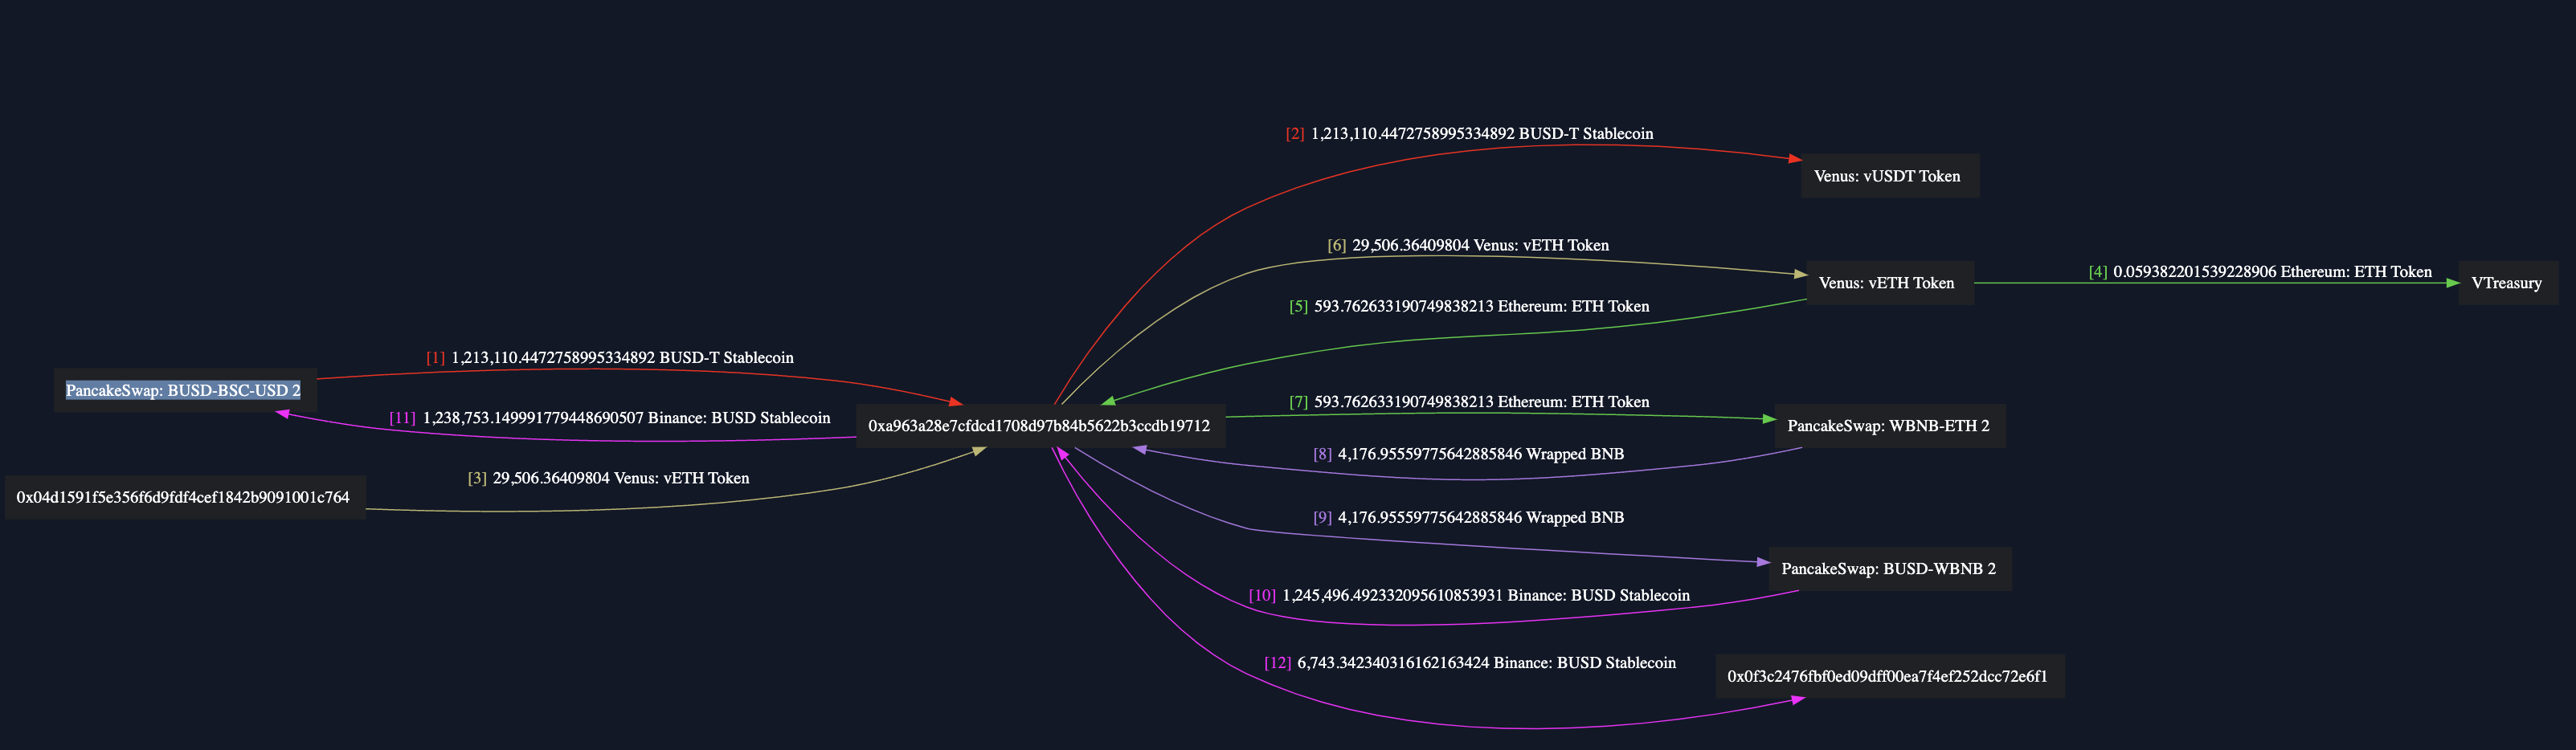
\includegraphics[scale=0.3]{img/liquidation_example.png}
  \caption{Tranzakcijos valiutų pavedimai \cite{liqpvz}}
  \label{img:liquidation_example}
\end{figure}

\begin{enumerate}
  \item \textbf{Trumpalaikė paskola.}  
  (1) pavedimu likvidatorius iš valiutų keityklos gauna 1213110 BUSD-T, su sąlyga, kad toje pačioje tranzakcijoje grąžins kitą valiutą – BUSD. Tai yra pirmasis žingsnis akimirksnio apsikeitimo (angl. \textit{flash swap}).

  \item \textbf{Likvidacijos veiksmai.}  
  (2) ir (3) pavedimais likvidatorius persiunčią visą prieš tai gautą BUSD-T į vUSDT baseiną, taip dalinai grąžindamas 0x04d... skolininko skolą. Mainais iš skolininko sąskaitos gauna vETH (\textit{Venus} protokolo apgaubtas ETH).

  \item \textbf{vETH konvertavimas į įprastą ETH.}  
  (5) ir (6) pavedimais likvidatorius išsikeičia turimus vETH į paprastą ETH, iš viso gaudamas 593,76 ETH.

  \item \textbf{ETH konvertavimas į BUSD.}  
  (7)--(10) pavedimais likvidatorius keičia ETH į BUSD tam, kad galėtų grąžinti trumpalaikę paskolą pirmajai keityklai. Po dviejų keitimų gauta 1245496 BUSD.

  \item \textbf{Skolos grąžinimas keityklai.}  
  Kadangi BUSD-T buvo gautas pirmajame pavedime, (11) pavedimu 
  grąžina 1238753 BUSD (maždaug 99,45\% iš (10) gautos sumos) pirmajai keityklai.

  \item \textbf{Pelnas likvidatoriui.}  
Po visų veiksmų likvidatoriaus piniginėje lieka 6743 BUSD, kurie (12-uoju pavedimu) pervedami į pelno piniginę.  
Kadangi BUSD prilygsta JAV doleriui, galutinės pajamos yra 6743 JAV doleriai.  
Sumokėjus 204 JAV dolerių tranzakcijos mokestį, likvidatoriui lieka 6539 JAV dolerių pelnas.
\end{enumerate}

\noindent
Jeigu likvidatoriui nereikėtų mokėti valiutų konvertavimo mokesčių, 
jam užtektų grąžinti apie 90,91\% (likvidacija grąžina 110\% įdėtos vertės) 
gauto užstato po likvidacijos. Tačiau realybėje egzistuoja tiek 
konvertavimo mokesčiai, tiek rinkos kainos gali skirtis nuo orakulo 
duomenų, todėl likvidatoriui teko grąžinti apie 99,45\% galutinės 
gautos valiutos.

\subsubsection{Atkartojimas}

\begin{table}[h!]
  \centering
  \caption{Reikšmės atkartojus likvidaciją}
  \begin{tabular}{|l|l|}
    \hline
    Mokestis už vieną kuro vienetą                           & 0,000000316441261625 BNB        \\
  \hline
  \multicolumn{2}{|c|}{\textbf{Likvidacija}}                              \\ \hline
  Grąžinta suma                            & 1213110,4472758995334892 BUSD-T         \\ \hline
  Užstato gauta \textit{wrapped} formatu             & 29506,36409804 vETH                     \\ \hline
  Kuro sunaudota dėl grąžinamos sumos patvirtinimo            & 24263                              \\ \hline
  Kuro sunaudota likvidacijos iškvietimui              & 816562                             \\ \hline
  Grąžinamos valiutos kaina               & 1,00148308 \$/BUSD-T               \\ \hline
  Užstato valiutos kaina          & 2250,50651698 \$/ETH            \\ \hline
  \multicolumn{2}{|c|}{\textbf{Užstato išsigryninimas (\textit{redeem})}}                                         \\ \hline
  \textit{Gas} sunaudota išsigryninimui                   & 141054                             \\ \hline
  Užstato gauta           & 593,762633190749838213 ETH             \\ \hline
  BNB kaina                & 298,22744081 \$/BNB             \\ \hline
  Pajamos                & \$121357,088416942287              \\ \hline
  Pelnas                 & \$121264,427054685937748              \\ \hline
  \end{tabular}
  \label{liquidation_example_repeat}
  \end{table}

\ref{liquidation_example_repeat} lentelėje pateikti skaičiai gauti pakartojus likvidaciją. Matome, kad pajamos yra 121 tūkstantis, kur \ref{img:liquidation_example} pav. pajamos yra tiktais 6,7 tūkstančiai. Šis skirtumas atsiranda iš to, kad orakulo kaina nesutampa su tuo ką gavo likvidatorius atliekant konvertavimus. Paimkime net pirmą konvertavimą po likvidacijos - ETH į BNB. Pagal orakulo kainas likvidatorius turėjo gauti 4\,480,7 BNB, tačiau gavo 4\,176,95 BNB (6,78\% mažiau). Tai gali būti tiek dėl orakulo ETH pervertinimo, o gal ETH-BNB keitykla tuo metu turėjo prastą kainą ir/arba mažą likvidumą. Pažymime, kad mūsų tyrimui šis skirtumas nėra svarbus, nes koncentruojamės tik į likvidacijos dalies optimizaciją ir proporciškai lyginame gautą užstatą.

\subsubsection{Strategijų lyginimas}
Toliau lyginamos skirtingos strategijos. Siekiant aiškiau suprasti situaciją, \ref{tab:strategijos_cf_analize} lentelėje pateikiama skolininko pradinė pozicija – nurodomos paskolos ir užstato valiutos, jų vertės bei atitinkami užstato koeficientai (CF). Remiantis \ref{liquidation_example_comp} lentelės duomenimis, matyti, kad originali likvidacija (\$1,21 mln.) buvo gerokai mažesnė nei maksimali galima suma (\$75,49 mln.) taikant strategiją \textit{iki uždarymo ribos}. Strategija \textit{didžiausia skola} sutampa su \textit{iki uždarymo ribos}, nes skolininko pozicijoje buvo tik viena pasiskolinta valiuta, o istorinis likvidatorius pasirinko likviduoti didžiausią užstatą – ETH. Naudojant orakulo teikiamas valiutų vertes, buvo galima pasiekti iki \$7{,}54 mln. pelną, tačiau tai reikalautų didelės apimties valiutų konvertavimo. Tokios operacijos reikalauja labai likvidžių rinkų, o siekiant išvengti reikšmingų kainų svyravimų, konvertavimą galimai tektų skaidyti per kelias rinkas. Pastebėtina, kad net ir originalus likvidatorius, konvertavęs tik \$1{,}21 mln. vertės turtą, jau susidūrė su nepalankiomis kainomis. Likusių rinkų likvidumo įvertinti negalime, nes tai reikalautų papildomos istorinės tų metų rinkų analizės.

Vis dėlto buvo galima likviduoti dar didesnį kiekį nei \$75,49 mln., pasinaudojus pasiūlyta \textit{pilno išeikvojimo} strategija. \ref{liquidation_example_comp} lentelėje šiai strategijai pateiktos dvi dalinės likvidacijos, išskirtos skolos grąžinimo ir užstato paėmimo stulpeliuose. Pirmosios likvidacijos dydis siekė \$36,27 mln., po jos skolininko sveikumo koeficientas ($HF$) turėjo likti šiek tiek mažesnis nei 1. Antroji likvidacija sudarė \$46,29 mln., tad bendra grąžinta skola iš viso siekė \$82,56 mln., o atitinkamai ir likvidatoriaus atlygis buvo proporcingai didesnis.

Iki šiol buvo aptariamos strategijos, kuriose tiek paskolos, tiek užstato valiutos buvo fiksuotos – pavyzdžiui, kai buvo likviduojama konkreti pora (\textit{USDT, ETH}). Taikant \textit{nuo didžiausio užstato koeficiento} strategiją, paskolos valiuta (USDT) išlieka fiksuota, tačiau atsiranda galimybė pasirinkti, kurią užstato valiutą likviduoti. 

Taikant \textit{nuo didžiausio užstato koeficiento} strategiją, buvo įvykdyti trys likvidacijos veiksmai, kiekvienas naudojant skirtingą užstato valiutą. Bendra sugrąžintos paskolos vertė siekė \$93{,}62 mln. – tai 13\,\% daugiau nei taikant \textit{pilno išeikvojimo} strategiją. Atidžiau išanalizavus matyti, kad \textit{pilno išeikvojimo} strategijoje naudotas užstatas visiškai sutampa su skolininko turimu ETH kiekiu. Tai reiškia, kad antroji likvidacija buvo apribota užstato kiekiu ir net nepasiekė uždarymo ribos. Vadinasi, apsiribojus vienos valiutos užstato likvidavimu, prarandama dalis galimo pelno. Priešingai, \textit{nuo didžiausio užstato koeficiento} strategija leidžia naudoti kelias užstato valiutas, todėl nėra apribojama konkrečios valiutos kiekiu, o likvidacija vyksta tol, kol pasiekiama uždarymo riba. Tokiu būdu ši strategija leidžia efektyviau išnaudoti skolininko užstatus ir generuoja didesnę grąžą.

Apie \textit{nuo didžiausio užstato koeficiento} atvejį dar galima pasakyti, kad XVS užstatas buvo nelikviduotas, nes jo vertė siekė tik apie 5 centus, o likvidacijos kvietimas būtų kainavęs daugiau nei gautas pelnas. Taip pat šiuo atveju visos skolininko pozicijoje esančios užstato valiutos turėjo vienodą užstato koeficientą (CF), todėl rikiavimas pagal koeficientą nedarė įtakos. Dėl to \textit{nuo mažiausio užstato koeficiento} strategija generavo identišką pelną kaip ir \textit{nuo didžiausio užstato koeficiento}.

\begin{table}[H]
\centering
\caption{Skolininko pradinė pozicija – skolos ir užstato duomenys}
\label{tab:strategijos_cf_analize}
\begin{tabular}{|c|c|c|c|}
\hline
\textbf{Valiuta} & \textbf{Skola (\$)} & \textbf{Užstatas (\$)} & \textbf{CF} \\ \hline
USDT &  150,97M   &  0        & 80\%  \\ \hline
XVS  &  0         &  0,05     & 80\%  \\ \hline
BTC  &  0         &  8,40M    & 80\%  \\ \hline
BNB  &  0         &  84,05M   & 80\%  \\ \hline
ETH  &  0         &  90,82M   & 80\%  \\ \hline
\end{tabular}
\end{table}

\begin{table}[h!]
  \centering
  \caption{Skirtingų likvidavimo strategijų rezultatai}
  \begin{tabular}{|>{\raggedright\arraybackslash}m{3.5cm}|>{\centering\arraybackslash}p{2cm}|>{\centering\arraybackslash}p{4cm}|c|c|}
  \hline
  \textbf{Strategija} & \textbf{Grąžinimas} & \textbf{Paimtas užstatas} & \textbf{Mokestis už kurą} & \textbf{Pelnas} \\ \hline
  Atkartoti                                    & \$1,21M   & 594 ETH (\$1,34M)     & 981 879 (\$92,66)    & \$121,26K \\ \hline
  Iki uždarymo ribos / Didžiausia skola        & \$75,49M & 36,9K ETH (\$83,03M) & 981 888 (\$92,66)    & \$7,54M   \\ \hline
  Pilnas išeikvojimas                & \makecell[c]{\$36,27M \\ \$46,29M \\ = \$82,56M}  & \makecell[c]{17,7K ETH (\$39,89M) \\ 22,6K ETH (\$50,92M) \\ = 40,3K ETH (\$90,81M)}  & 1 630 707 (\$153,89) & \$8,25M   \\ \hline
  Nuo didžiausio/mažiausio užstato koeficiento & \makecell[c]{\$7,6M \\ \$28,6M \\ \$57,3M \\ = \$93,62M}  &  \makecell[c]{231 BTC (\$8,40M) \\ 105K BNB (\$31,49M) \\ 28K ETH (\$63,07M) \\ = \$102,97M}    & 2 665 850 (\$251.58)   & \$9,35M   \\ \hline
  \end{tabular}
  \label{liquidation_example_comp}
  \end{table}

\subsection{Pilnas išeikvojimas vienodoms valiutoms}
\label{sec:pilnas_iseikvojimas_vienodoms_valiutoms_tyrimas}

Parodome, kad \textit{pilno išeikvojimo} strategija gali būti efektyvesnė nei primityvioji \textit{didžiausios skolos} strategija, kartu eliminuojant valiutos likvidumo klausimą. Šiame skyriuje analizuojame tik tuos atvejus, kai skolos grąžinimo ir užstato valiutos sutampa, todėl pelnas taip pat išreiškiamas ta pačia valiuta. Tokį apribojimą motyvuoja tai, kad sudėtingesnė \textit{pilnas išeikvojimo} strategija leidžia grąžinti didesnę skolos dalį ir atgauti didesnę užstato sumą, kas dažnai reikalauja didelius valiutų keitimo kitose rinkose. Tačiau didesni keitimo kiekiai lemia didesnį kainos pokytį nepalankia kryptimi. Taigi, nors iš vienos pusės optimizuojamas likvidacijos dydis, kartu patiriamas ir didesnis kainos nuokrypis, galintis sumažinti arba visiškai panaikinti pelno augimą. Todėl šio skyriaus analizėje koncentruojamės į scenarijus, kuriuose valiutų keitimas nėra būtinas. Išimtį sudaro atvejai, kai likvidatoriui pelnas pageidaujamas konkrečia valiuta – tuomet atliekami valiutų keitimai, tačiau jų apimtis gerokai mažesnė, nes keičiamas tik pelnas, t. y. apie 10\% grąžintos skolos dydžio.

Arbitražo vykdymo kontekste likviduojama valiuta nebūtinai yra ta, kurią likviduotojas ketina laikyti ilgesnį laiką. Todėl, įvykdęs likvidaciją, likviduotojas gali gautą pelną ta valiuta konvertuoti į stabilesnę, pavyzdžiui, USDC, kuris yra susietas su JAV doleriu. Šis konvertavimą galima atlikti atskiroje tranzakcijoje, kurios kuro mokestis už vienetą yra mažesnis nei pačios likvidacijos metu.

Didelis kuro mokestis likvidacijos tranzakcijai gali būti nustaytas dėl kelių priežasčių. Viena priežastis – noras būti greičiau įtrauktam į bloką arba būti pirma tranzakcija bloke. Kita priežastis – pasinaudoti blokų grandinės tranzakcijų rikiavimo logika: nustatant aukštesnį kuro mokestį galima valdyti tranzakcijos vietą bloke, siekiant, kad ji būtų iškart po kitos tranzakcijos, sukuriančios likvidacijos galimybę, pavyzdžiui, orakulo kainos atnaujinimo.

Kalbant apie skolos grąžinimą, būtina turėti kapitalo, reikalingo skolai padengti. Šį kapitalo prieinamumo klausimą sprendžia įvairios rinkos, leidžiančios momentiškai (per \textit{flash loan}) pasiskolinti konkrečią valiutą už tam tikrą mokestį. Taigi, pasitelkus šias priemones ir technikas, galima vykdyti likvidacijas su minimalia rizika bei gauti pelną.

\subsubsection{Pelningiausias atvejis}

% SELECT (drain_same_token->>'profit_usd')::NUMERIC, transaction_hash, drain_same_token, created_at
% FROM bsc.venus_liquidation_tests
% WHERE TRUE
% AND (drain_same_token->>'profit_usd')::NUMERIC > 0
% ORDER BY 1 DESC

Iš išanalizuotų likvidacijų identifikuotas pelningiausias \textit{pilno išeikvojimo vienodoms valiutoms} strategijos atvejis. Analizuojame tranzakciją \\ \texttt{0xcebfe3ec5782ad5f1a52f3727c3986abb1f2314cd1c0f0baf18ec20e1000fea9}.

\ref{tab:drain_same_token_position_most} lentelėje pateikta skolininko pozicija – ji sudaryta tik iš DOGE valiutos. Dėl šios priežasties daugelio strategijų veiksmai sutampa. \ref{tab:drain_same_token_profit_most} lentelėje pateikti skirtingų strategijų pelnai.

Šiuo atveju originalus likvidatorius likvidavo iki uždarymo ribos, todėl jo pelnas sutampa su \textit{iki uždarymo ribos} strategijos rezultatu. \textit{Didžiausia skola} strategija taip pat duoda tokį patį rezultatą, kadangi nėra kitų galimų valiutų porų (tik DOGE-DOGE).

\textit{Pilno išeikvojimo} strategijai pavyko likviduoti didesnį kiekį skolos nei paprastai \textit{iki uždarymo ribos} strategijai, todėl ji uždirbo apie 20\% didesnį pelną. Kaip matyti ir iš lentelės, skolininko sveikumo koeficientas ($HF$) po likvidacijos buvo gerokai aukštesnis, todėl ši strategija pasirodė efektyvesnė likviduojant kuo didesnę skolos dalį.

\begin{table}[H]
\centering
\caption{Pradinė skolininko pozicija}
\label{tab:drain_same_token_position_most}
\begin{tabular}{|c|c|c|c|c|}
\hline
\textbf{Valiuta} & \textbf{Skola (\$)} & \textbf{Užstatas (\$)} & \textbf{CF} & \textbf{HF} \\ \hline
DOGE &  2 617 497   &  5 822 673       & 40\% & 0,889 \\ \hline
\end{tabular}
\end{table}

\begin{table}[h!]
  \centering
  \caption{Skirtingų likvidavimo strategijų rezultatai}
  \begin{tabular}{|>{\raggedright\arraybackslash}m{3.5cm}|>{\centering\arraybackslash}p{2.9cm}|>{\centering\arraybackslash}p{2.5cm}|>{\centering\arraybackslash}p{2.5cm}|c|>{\centering\arraybackslash}p{2cm}|}
  \hline
  \textbf{Strategija} & \textbf{Grąžinimas} & \textbf{Paimtas užstatas} & \textbf{Mokestis už kurą} & \textbf{Pelnas} & \textbf{Galutinis $HF$} \\ \hline
  Atkartoti & \$1,308M   & \$1,439M     & \$104    & \$130K & 1.339 \\ \hline
  Iki uždarymo ribos / Didžiausia skola & \$1,308M   & \$1,439M     & \$104    & \$130K & 1.339 \\ \hline
  Pilnas išeikvojimas / Pilnas išeikvojimas vienodoms valiutoms & \makecell[c]{\$515K \\ \$1,051M \\ = \$1,566M}   & \makecell[c]{\$566K \\ \$1,156M \\ = \$1,722M}     & \$171    & \$156K & 1.56  \\ \hline
  \end{tabular}
  \label{tab:drain_same_token_profit_most}
  \end{table}

% \subsubsection{Kitas atvejis}
% % SELECT
% % (large_borrow ->>'profit_usd')::NUMERIC AS largest_loan_profit,
% % (drain_same_token->>'profit_usd')::NUMERIC AS same_token_profit,
% % transaction_hash, drain_same_token, created_at
% % FROM bsc.venus_liquidation_tests
% % WHERE TRUE
% % AND (drain_same_token->>'profit_usd')::NUMERIC > 10000
% % AND (large_borrow ->>'profit_usd')::NUMERIC  > 0
% % ORDER BY (drain_same_token->>'profit_usd')::NUMERIC / (large_borrow ->>'profit_usd')::NUMERIC  DESC

% % SELECT * FROM bsc.venus_liquidation_tests
% % WHERE transaction_hash = '0x67cc58e0d8e2ddd8eea396fb3e667bf4ba295541b1d8d3d2ee600529a1f26138'
% % ORDER BY created_at desc

% \begin{table}[H]
% \centering
% \caption{Pradinė skolininko pozicija}
% \label{tab:drain_same_token_position_ratio}
% \begin{tabular}{|c|c|c|c|c|}
% \hline
% \textbf{Valiuta} & \textbf{Skola (\$)} & \textbf{Užstatas (\$)}  \\ \hline
% ETH  &  0        &  235\,783 \\ \hline
% USDC &  199\,502 &  200\,153 \\ \hline
% BNB  &  0        &  99\,184  \\ \hline
% XVS  &  0        &  19\,109  \\ \hline
% BUSD &  0        &  0,06     \\ \hline
% DAI  &  151\,329 &  0        \\ \hline
% USDT &  109\,419 &  0        \\ \hline
% FIL  &  47       &  0        \\ \hline
% \end{tabular}
% \end{table}

% Nupiesiame pelno lentele, parodome, kad 

\subsubsection{Bendras pelnas}
\label{sec:drain_bendras_pelnas}
% SELECT count(*) AS total_liquidations,
% count(*) FILTER (WHERE (drain_same_token->>'profit_usd')::NUMERIC > 0) AS drain_same_token_profitable,
% count(*) FILTER (WHERE (drain_same_token->>'profit_usd')::NUMERIC > (large_borrow->>'profit_usd')::NUMERIC) AS drain_same_token_more_profitable_than_largest_borrow
% FROM bsc.venus_liquidation_tests

Iš viso išanalizuota 25\,042 likvidacijų. Iš jų 2\,571 atvejais strategija \textit{pilnas išeikvojimas vienodoms valiutoms} buvo pelninga. Iš šių atvejų 337 parodė didesnį pelną nei strategija \textit{didžiausia skola}.

Vertinant bendrą pelną pasirinktai strategijai, būtų klaidinga kiekvieną įvykusią likvidaciją analizuoti atskirai, apskaičiuoti pelną pagal pasirinktą strategiją ir šiuos rezultatus tiesiog sumuoti. Kaip matyti iš \ref{liquidation_example_comp} lentelės, istoriniuose duomenyse ne visi likvidatoriai maksimaliai išnaudojo turimą likvidacijos potencialą, o didesnės galimybės dažnai būna išskaidytos į daugybę mažesnių likvidacijų. Dėl to būtų klaidinga sumuoti pelnus kiekvienai atskirai likvidacijai, nes geresnės strategijos atveju tas pats pelnas gali būti įtrauktas kelis kartus. Problema kyla dėl to, kad viena likvidacija gali turėti įtakos kitoms, su ja susijusioms likvidacijoms – modifikuodami vieną iš jų, galime netiesiogiai pakenkti kitoms. Savo tyrime kiekvieną atvejį analizuojame izoliuotai, neatsižvelgdami į jų tarpusavio sąveikas. Dažniausias ryšys tarp skirtingų likvidacijų yra tas pats skolininkas. Kiti galimi priklausomumai – likvidacija, kuri išnaudoja visą likusį grynųjų likutį iš \textit{Venus} valiutų baseino, atima galimybę išsigryninti kitiems dalyviams; arba vieno likvidatoriaus veiksmai sumažina rinkos likvidumą, apsunkindami valiutų keitimą kitiems.

% WITH most_profitable_liquidation_tests AS (
%     SELECT DISTINCT ON (borrower) *
%     FROM bsc.venus_liquidation_tests
%     JOIN bsc.venus_liquidations USING(transaction_hash)
%     WHERE (drain_same_token ->> 'profit_usd')::NUMERIC > 0
%     ORDER BY borrower, (drain_same_token ->> 'profit_usd')::NUMERIC DESC
% ),
% assets AS (
%     SELECT 
%       transaction_hash, jsonb_array_elements(drain_same_token->'assets') AS asset
%     FROM most_profitable_liquidation_tests 
%     WHERE TRUE
%     AND (drain_same_token ->>'profit_usd')::NUMERIC  > 0
% ),
% aggregated_assets AS (
%     SELECT
%     asset->'initial_data'->>'symbol' AS symbol,
%     sum((asset->>'collateral_underlying_gained')::NUMERIC) AS collateral_gained,
%     sum((asset->>'repaid')::NUMERIC) AS repaid,
%     sum((asset->>'collateral_underlying_gained')::NUMERIC - (asset->>'repaid')::NUMERIC) AS profit_underlying,
%     sum(((asset->>'collateral_underlying_gained')::NUMERIC - (asset->>'repaid')::NUMERIC) * (asset->'initial_data'->>'price')::NUMERIC / 1e36) AS profit_usd,
%     sum((asset->>'liquidations_participated')::NUMERIC) AS liquidations_participated
%     FROM assets a
%     WHERE (asset->>'collateral_underlying_gained')::NUMERIC > 0
%     AND (asset->>'repaid')::NUMERIC > 0
%     GROUP BY asset->'initial_data'->>'symbol'
% )
% --,res AS (
% SELECT
%     symbol,
% --    collateral_gained,
% --    repaid,
% --    profit_underlying,
%     profit_usd,
%     liquidations_participated
% FROM aggregated_assets a
% ORDER BY profit_usd DESC

% )
% SELECT sum(profit_usd) FROM res

Siekiant įvertinti strategijos \textit{pilnas išeikvojimas vienodoms valiutoms} bendrą pelningumą tais atvejais, kai tam pačiam skolininkui galimi keli likvidacijos įvykiai, taikomas apribojimas: kiekvienam skolininkui pelno skaičiavime įtraukiamas tik vienas – pelningiausias – įvykis. Pritaikius šį apribojimą, pelningų įvykių skaičius sudaro 1\,317 iš 2\,571 visų identifikuotų pelningų atvejų. Atrinktų įvykių rezultatai pateikti \ref{tab:liq_same_tokens_profit} lentelėje, kurioje nurodomas bendras pelnas, gautas kiekvienoje atskiroje valiutoje. Valiutos vertei nustatyti daroma prielaida, kad gauta pelno suma realizuota pagal tuo metu galiojusią orakulo kainą, o sandorių mokesčiai yra nereikšmingi. Bendra teorinė grąža sudaro apie 1,4 mln.\ JAV dolerių, tai yra tiek būtų buvę galima uždirbti vykdant likvidacijas, kai grąžinimo ir atsiimamo užstato valiutos sutampa. Tokiu būdu išvengiama valiutų konvertavimo operacijų, kurios galėtų būti nuostolingos dėl kainų nepastovumo, bei su tuo susijusių papildomų mokesčių – tiek valiutų keitimo mokesčių, tiek kuro sąnaudų, ypač esant aukštoms \textit{gas} kainoms.

% WITH most_profitable_liquidation_tests AS (
%     SELECT DISTINCT ON (borrower) *
%     FROM bsc.venus_liquidation_tests
%     JOIN bsc.venus_liquidations USING(transaction_hash)
%     WHERE (drain_same_token ->> 'profit_usd')::NUMERIC > 0
%     ORDER BY borrower, (drain_same_token ->> 'profit_usd')::NUMERIC DESC
% )
% SELECT
% count(*),
%     sum((drain_same_token ->>'profit_usd')::NUMERIC) AS drain_total_profit,
%     sum((large_borrow ->>'profit_usd')::NUMERIC) AS largest_borrow_total_profit
% FROM most_profitable_liquidation_tests 
% WHERE TRUE
% AND (drain_same_token ->>'profit_usd')::NUMERIC > (large_borrow ->>'profit_usd')::NUMERIC

Norint kiekybiškai įvertinti \textit{pilno išeikvojimo vienodoms valiutoms} strategijos pranašumą prieš \textit{didžiausios skolos} metodą, analizuojami tik tie atvejai, kuriuose pirmoji strategija generuoja didesnį pelną. Iš 337 tokių atvejų, 94 susiję su unikaliais skolininkų adresais, todėl tolesnėje analizėje vertinami tik pelningiausi 94 įvykiai — po vieną kiekvienam skolininkui. Šioje imtyje \textit{pilno išeikvojimo vienodoms valiutoms} strategija sugeneravo bendrą \$606\,398 pelną, o \textit{didžiausios skolos} metodas – tik \$546\,117. Gauti rezultatai empiriškai patvirtina, kad išplėstinė strategija gali būti finansiškai pranašesnė, kartu eliminuojant valiutų keitimo problematiką, kurios įtaka dažniausiai ryškesnė taikant \textit{pilno išeikvojimo} strategiją.

\begin{table}[H]
\centering
\caption{\textit{Pilnas išeikvojimas vienodoms valiutoms} pelnas pagal valiutą}
\label{tab:liq_same_tokens_profit}
\begin{tabular}{|l|r|r|}
\hline
\textbf{Valiuta} & \textbf{Valiutos vertė (\$)} & \textbf{Likvidacijų kvietimai} \\
\hline
DOGE  & 333\,188,40  & 21 \\
BUSD  & 280\,728,73  & 301 \\
SXP   & 169\,691,27  & 57 \\
ETH   & 134\,977,21  & 120 \\
DAI   & 119\,947,04  & 26 \\
BTC   & 91\,450,61   & 173 \\
USDT  & 85\,647,06   & 321 \\
BNB   & 81\,680,97   & 374 \\
USDC  & 80\,301,13   & 174 \\
XVS   & 20\,878,56   & 14 \\
MATIC & 12\,799,84   & 10 \\
AAVE  & 8\,226,96    & 7 \\
DOT   & 1\,654,70    & 19 \\
XRP   & 1\,519,91    & 23 \\
ADA   & 1\,145,77    & 17 \\
BETH  & 899,91     & 30 \\
CAKE  & 895,97     & 11 \\
BCH   & 614,01     & 5 \\
WBETH & 484,21     & 2 \\
CAN   & 349,34     & 9 \\
FIL   & 135,10     & 5 \\
LTC   & 89,87      & 11 \\
LINK  & 60,36      & 8 \\
TRX   & 50,41      & 1 \\
TRXOLD & 43,02     & 8 \\
UST   & 24,71      & 1 \\
TUSD  & 3,79       & 1 \\
\hline
\end{tabular}
\end{table}

% \subsection{Nuo didžiausio užstato koeficiento}
% \textcolor{red}{
% Palyginti "nuo didžiausio" ir "nuo mažiausio". Turėtų būti skirtumas kai skolininko pozicijos turi valiutų su skirtingais koeficientais.
% }

\subsection{Strategijų vertinimas remiantis dideliais duomenų rinkiniais}
\label{sec:lyginimas_daug}

Norint įvertinti likvidavimo strategijų efektyvumą ne pavieniais atvejais, bet sistemingai – būtina atlikti analizę remiantis plačiu istorinių duomenų rinkiniu. Tik tokiu būdu galima įžvelgti bendras tendencijas, įvertinti strategijų stabilumą įvairiose rinkos sąlygose ir išskirti atvejus, kai vieni metodai ženkliai pranašesni už kitus.

Susiduriame su panašia problema kaip ir \ref{sec:drain_bendras_pelnas} poskyryje – negalime tiesiog eiti chronologine tvarka ir sumuoti pelno, nes pelningesnės strategijos kartais tą pačią likvidavimo galimybę išnaudoja kelis kartus. Šįkart, kaip ir anksčiau, į analizę įtraukiama tik viena kiekvieno skolininko likvidacija, tačiau siekiant išvengti šališkumo kuriai nors strategijai, pasirenkama pati pirmoji kiekvieno skolininko likvidacija. Taikant šį kriterijų, gaunami 10\,068 įvykiai iš viso 63\,982 analizuotų likvidacijų (15,73\%). Kiekvienam įvykiui atlikus analizę, kaip pavaizduota \ref{liquidation_example_comp} lentelėje, ir sukaupus pelno reikšmes chronologine tvarka (pagal blokus), gaunami rezultatai, pateikti \ref{img:bendras2} paveiksle.

% WITH first_borrower_liquidations AS (
%     SELECT DISTINCT ON (borrower) *
%     FROM bsc.venus_liquidation_tests
%     JOIN bsc.venus_liquidations USING(transaction_hash)
%     ORDER BY borrower, block_number ASC, transaction_index ASC
% ),
% profits AS (
%     SELECT
%         transaction_hash,
%         borrower,
%         block_number,
%         transaction_index,
%         (repeat->>'profit_usd')::NUMERIC AS repeat,
%         (up_to_close_factor->>'profit_usd')::NUMERIC AS up_to_close_factor,
%         (drain->>'profit_usd')::NUMERIC AS drain,
%         (large_borrow->>'profit_usd')::NUMERIC AS large_borrow,
%         (drain_same_token->>'profit_usd')::NUMERIC AS drain_same_token,
%         (largest_cf_first->>'profit_usd')::NUMERIC AS largest_cf_first,
%         (smallest_cf_first->>'profit_usd')::NUMERIC AS smallest_cf_first
%     FROM first_borrower_liquidations
% )
% SELECT
%     transaction_hash,
%     borrower,
%     block_number,
%     repeat,
%     SUM(repeat) OVER (ORDER BY block_number, transaction_index) AS repeat_accumulated,
%     up_to_close_factor,
%     SUM(up_to_close_factor) OVER (ORDER BY block_number, transaction_index) AS up_to_close_factor_accumulated,
%     drain,
%     SUM(drain) OVER (ORDER BY block_number, transaction_index) AS drain_accumulated,
%     large_borrow,
%     SUM(large_borrow) OVER (ORDER BY block_number, transaction_index) AS large_borrow_accumulated,
%     drain_same_token,
%     SUM(drain_same_token) OVER (ORDER BY block_number, transaction_index) AS drain_same_token_accumulated,
%     largest_cf_first,
%     SUM(largest_cf_first) OVER (ORDER BY block_number, transaction_index) AS largest_cf_first_accumulated,
%     smallest_cf_first,
%     SUM(smallest_cf_first) OVER (ORDER BY block_number, transaction_index) AS smallest_cf_first_accumulated
% FROM profits
% ORDER BY block_number asc, transaction_index asc;

\begin{figure}[H]
  \centering
  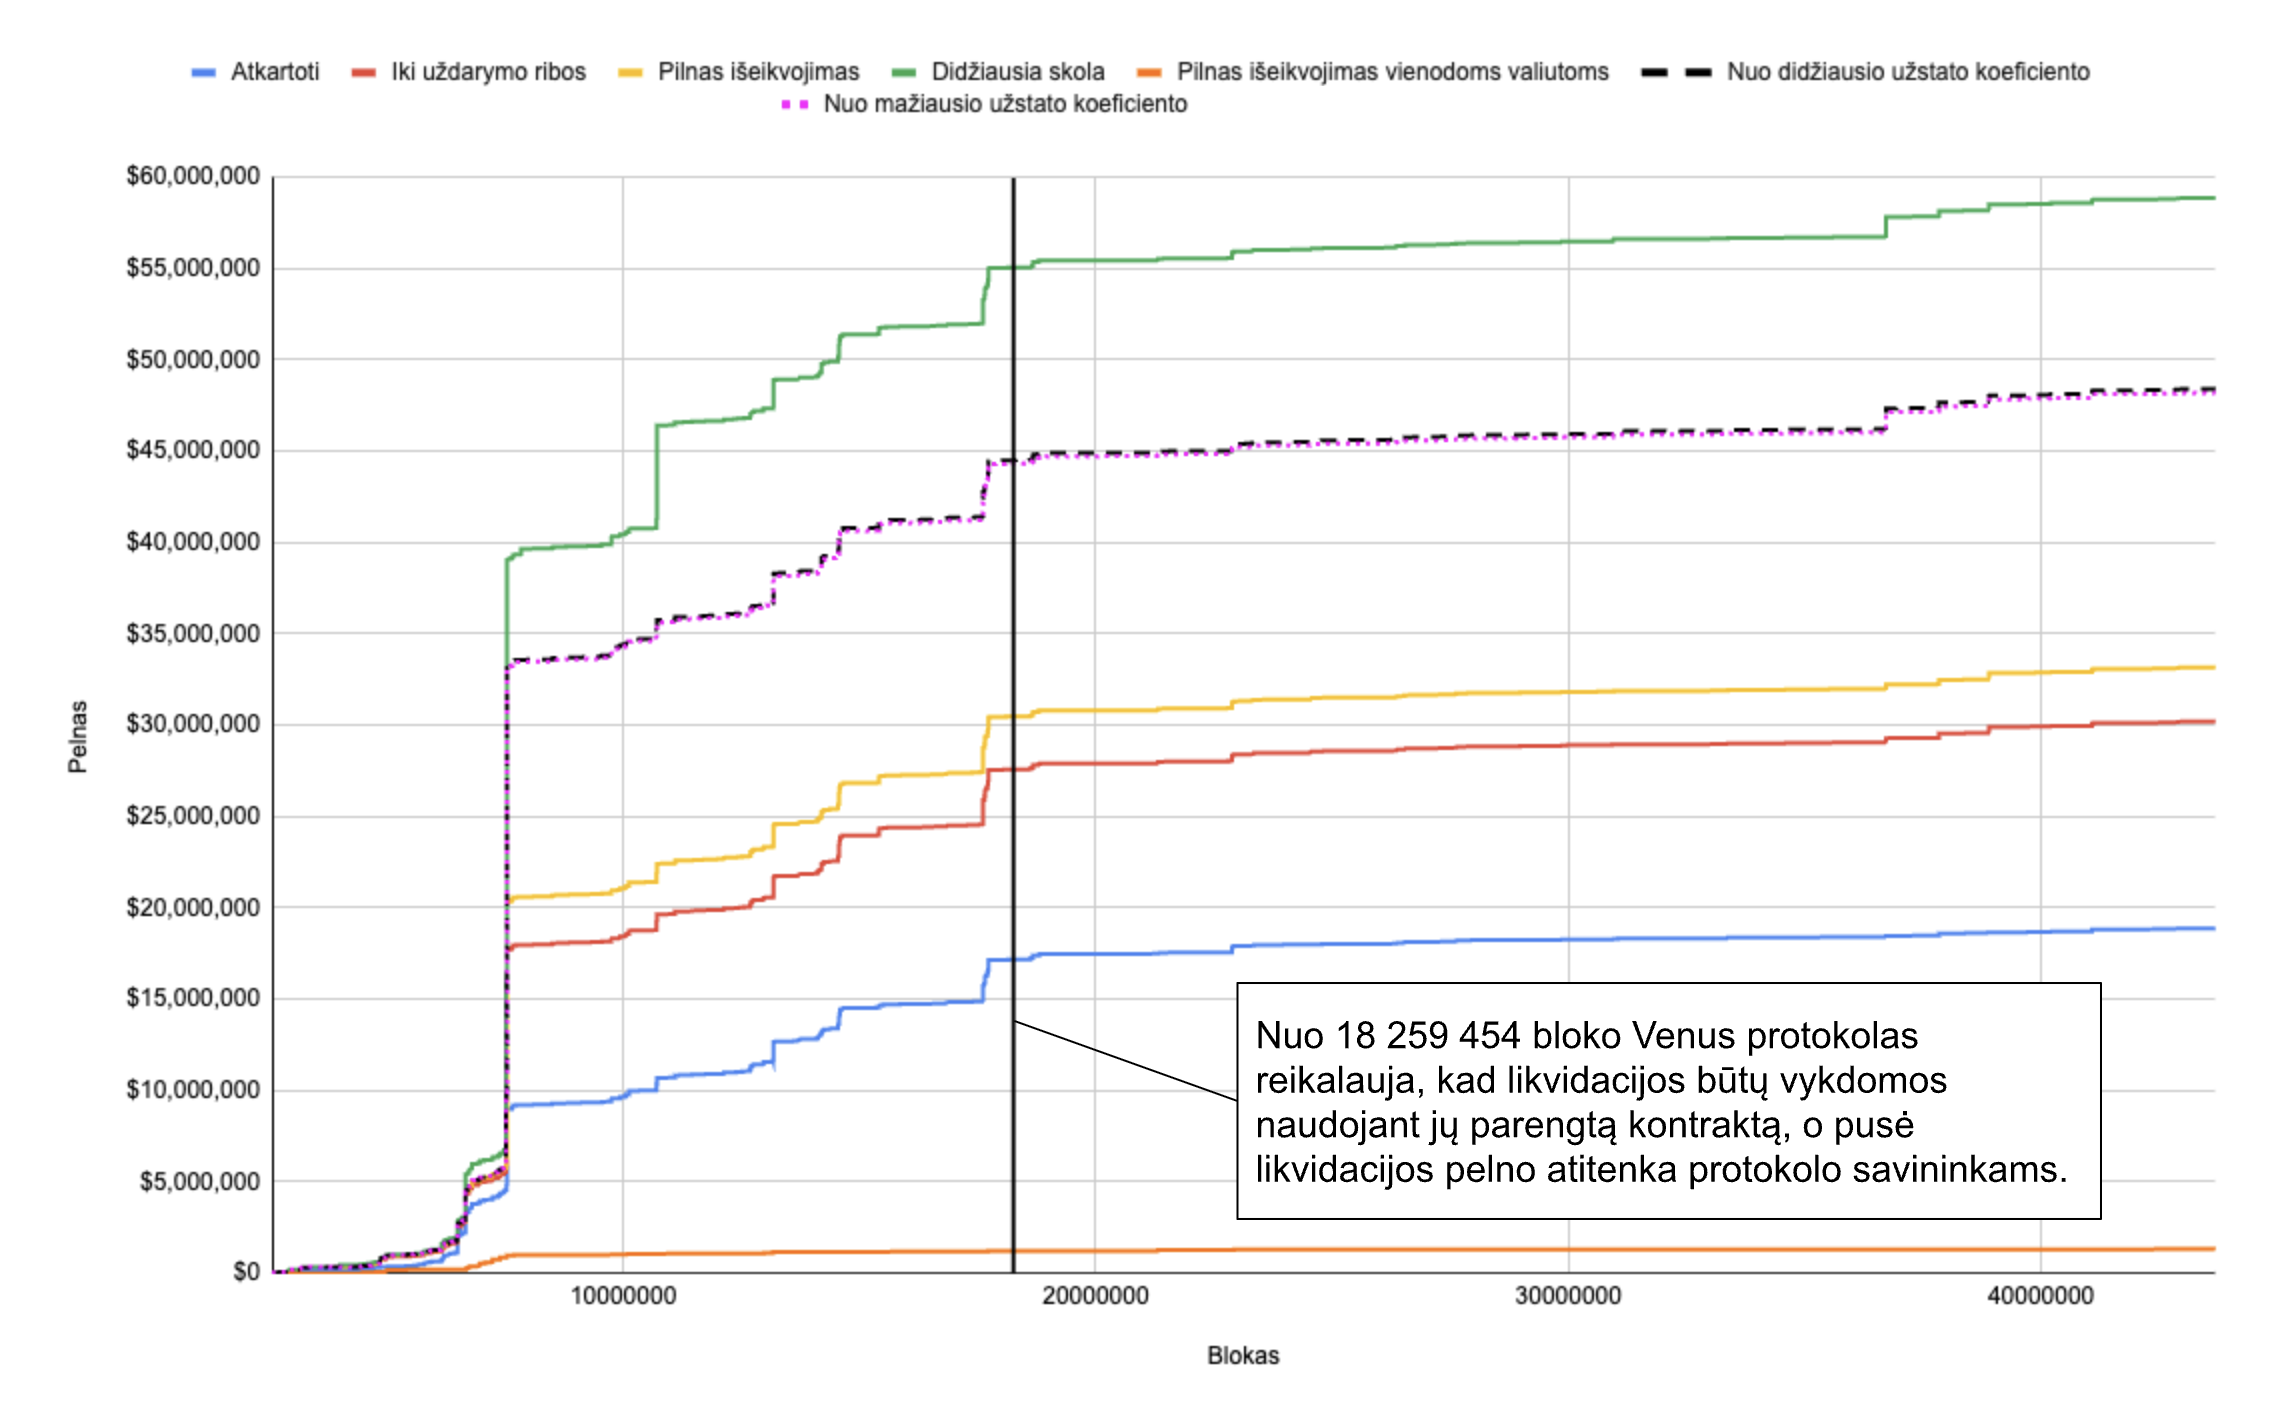
\includegraphics[scale=0.4]{img/bendras5.png}
  \caption{Kaupiamasis pelnas pagal strategijas, atsižvelgiant tik į pirmąją kiekvieno skolininko likvidaciją}
  \label{img:bendras2}
\end{figure}

\begin{table}[h!]
  \centering
  \caption{Strategijų pelnai}
  \label{tab:strategiju_pelnai}
  \begin{tabular}{|l|r|}
  \hline
  \textbf{Strategija} & \textbf{Pelnas (\$)} \\ \hline
  Atkartoti                               & 18\,884\,165 \\ \hline
  Iki uždarymo ribos                      & 30\,196\,914 \\ \hline
  Pilnas išeikvojimas                     & 33\,158\,449 \\ \hline
  Didžiausia skola                        & 58\,856\,203 \\ \hline
  Pilnas išeikvojimas vienodoms valiutoms & 1\,319\,302  \\ \hline
  Nuo didžiausio užstato koeficiento      & 48\,409\,265 \\ \hline
  Nuo mažiausio užstato koeficiento       & 48\,198\,907 \\ \hline
  \end{tabular}
  \end{table}

Pirmiausia analizuojamos strategijos, kurių skolos ir užstato valiutos yra fiksuotos. Tarp jų – \textit{atkartojimo}, \textit{iki uždarymo ribos} bei \textit{pilno išnaudojimo} strategijos. Rezultatai, pateikti \ref{tab:strategiju_pelnai} lentelėje, rodo, kad taikant \textit{iki uždarymo ribos} strategiją pasiektas pelnas buvo 59,9\% didesnis nei naudojant \textit{atkartojimo} strategiją, o \textit{pilno išnaudojimo} strategijos atveju pelnas viršijo \textit{atkartojimo} strategijos rezultatus net 75,5\%. Šie rezultatai leidžia daryti prielaidą, kad reikšminga dalis prarasto pelno istoriniuose duomenyse yra susijusi su tuo, jog likvidatoriai dažnai negrąžina visos maksimaliai leidžiamos sumos. Vis dėlto net ir laikantis tokių pačių valiutų porų likvidacijose, galima identifikuoti maždaug 9,8\% papildomo pelno potencialą, taikant efektyvesnius sprendimus.

Suteikus galimybę rinktis skirtingas užstato valiutas, pastebimas pelningumo augimas. Strategijos \textit{nuo didžiausio užstato koeficiento} ir \textit{nuo mažiausio užstato koeficiento} atitinkamai generavo \$48,409 mln. ir \$48,198 mln. pelno. Kadangi šiose strategijose skolos valiuta išlaikoma nepakitusi, galima teigti, kad pelno augimą lėmė efektyvesnis likviduojamo skolininko užstatų panaudojimas. Be to, \textit{nuo didžiausio užstato koeficiento} strategija pasižymėjo 0,436\% didesniu pelnu nei alternatyvi, o tai patvirtina darbo \ref{sec:from_largest_cf} skyriuje išvystą teiginį, jog didesnio užstato koeficiento užstatų likvidavimas pirmiausia yra ekonomiškai naudingesnis. Tačiau reikšmingas skirtumas tarp \textit{pilno išnaudojimo} ir \textit{nuo didžiausio užstato koeficiento} strategijų rezultatų bei mažas skirtumas tarp \textit{nuo didžiausio užstato koeficiento} ir \textit{nuo mažiausio užstato koeficiento} leidžia daryti išvadą, kad didesnę įtaką turi skirtingų užstato valiutų išnaudojimas, o ne jų pasirinkimo tvarka.

Didžiausią pelningumą demonstravo strategija \textit{didžiausia skola}. Nors šioje strategijoje apribota likvidacijos kvietimų skaičius iki vieno, ji išsiskiria tuo, kad leidžia pasirinkti grąžinamą valiutą. Tai, kad \textit{didžiausios skolos} strategijos pelnas buvo 94,9\% didesnis nei \textit{iki uždarymo ribos}, rodo, jog istoriniai likvidatoriai ne visuomet renkasi optimalias skolos ir užstato valiutas pagal jų vertę. Taip pat 21,5\% didesnis pelnas nei \textit{nuo didžiausio užstato koeficiento} strategijoje leidžia manyti, jog pastaroji strategija turi papildomo pelno potencialą, jeigu joje būtų sprendžiamas ir skolos valiutos pasirinkimo klausimas. Šiame darbe, \textit{nuo didžiausio užstato koeficiento} strategijoje buvo sąmoningai apsiribota tik užstato valiutos pasirinkimu.

Galiausiai, \textit{pilno išnaudojimo} strategija, taikoma vienodoms valiutų poroms, generavo \$1,319 mln. pelno – tai yra 5,7\% mažiau nei \ref{sec:drain_bendras_pelnas} skyriuje nurodytas \$1,4 mln. pelnas. Šis skirtumas paaiškinamas atrankos kriterijais: šiame skyriuje nagrinėjami tik tie įvykiai, kai skolininkas likviduojamas pirmą kartą, o ankstesniame skyriuje – pelningiausi kiekvieno skolininko įvykiai pagal šią strategiją.

Nuo 18259454 \cite{LikvidacijosKontraktas} bloko \textit{Venus} protokolas pakeitė likvidavimo mechanizmą. Po pakeitimo visos likvidacijos privalo būti vykdomos per \textit{Venus} protokolo parengtą kontraktą, kuris pasilieka pusę likvidacijos pelno, 5\% nuo likviduojamos sumos, ir kitus 5\% atiduoda likvidatoriui. Po šio pakeitimo pastebimas reikšmingas pelno lėtėjimas, tačiau tai taip pat gali būti susiję su tuo, kad laikui bėgant į grafiką patenka vis mažiau likvidacijų, nes analizuojame tik po vieną likvidaciją vienam skolininkui.

\subsubsection{Išskirtiniai atvejai}
Galime atkreipti dėmesį, kad \ref{img:bendras2} pav. visų strategijų pelno kreivės yra panašios, jei atmesime kelis išskirtinius staigius šuolius tam tikruose laiko momentuose. Tai reiškia, kad strategijų pelno skirtumą smarkiai veikia keletas įvykių. Blokų ruože 7544850–7546511 įvyko trys didelės likvidacijos, kurių metu pastebėtas reikšmingas skirtumas tarp strategijų:

\begin{enumerate}[label=\textbf{\Alph*.}]
    \item \texttt{0x0cd0fc0cdd5b572d71cd039cc522d20dfcc5c8c0772173b484c91194401fe89b}
    \item \texttt{0x718cf2813f3124f576a64a69429ec543ea6b14ca53d557772d61e72a6c256f3e}
    \item \texttt{0x3b04a03ed356108c7297e6b438d70df7383f10d39d0511603b576b635d6bff9f}
\end{enumerate}

% Įdomu yra tai, kad visi trys nagrinėjami atvejai išsiskiria savo duomenimis dėl skirtingų priežasčių. 
\ref{tab:profit_table} lentelėje nurodome, kokį pelną kiekvienoje situacijoje generavo kiekviena strategija.

\begin{table}[H]
  \centering
  \caption{Strategijų pelno palyginimas (skliaustuose likvidacijų iškvietimų skaičius)}
  \label{tab:profit_table}
  \begin{tabular}{|l|c|c|c|}
  \hline
  \textbf{Strategija} & \textbf{A} & \textbf{B} & \textbf{C} \\ \hline
  Atkartoti                               & \$2\,015\,683 (1)  & \$190\,227 (1)     & \$15\,074 (1)      \\ \hline
  Iki uždarymo ribos                      & \$2\,015\,683 (1)  & \$6\,630\,951 (1)  & \$1\,060\,317 (1)  \\ \hline
  Pilnas išeikvojimas                     & \$4\,031\,326 (20) & \$6\,630\,951 (1)  & \$1\,083\,910 (2)  \\ \hline
  Didžiausia skola                        & \$4\,778\,392 (1)  & \$12\,710\,977 (1) & \$1\,060\,317 (1)  \\ \hline
  Pilnas išeikvojimas vienodoms valiutoms & \$0 (0)            & \$0 (0)            & \$0 (0)            \\ \hline
  Nuo didžiausio užstato koeficiento      & \$4\,031\,319 (22) & \$12\,793\,976 (2) & \$1\,083\,910  (2) \\ \hline
  Nuo mažiausio užstato koeficiento       & \$4\,031\,319 (22) & \$12\,793\,976 (2) & \$1\,083\,910 (2)  \\ \hline
  \end{tabular}
\end{table}

\paragraph{A atvejis}

Pirmuoju atveju (žr. \ref{case_a} lentelę) originalioje tranzakcijoje likvidatorius grąžino skolą BUSD valiuta, naudodamas maksimalią leistiną sumą vieno likvidavimo funkcijos iškvietimo metu. Dėl šios priežasties \textit{atkartoti} ir \textit{iki uždarymo ribos} strategijų sugeneruotas pelnas sutapo. Šiame scenarijuje skolininkas turėjo reikšmingą įsiskolinimą, todėl \textit{pilno išeikvojimo} strategijoje buvo galima inicijuoti iki 50 likvidavimo kvietimų, kiekvieno jų metu grąžinant dvigubai mažesnę sumą nei ankstesnėje iteracijoje. Nuo 21-os iteracijos likvidavimo kvietimai tampa ekonomiškai neefektyvūs, kadangi jų pelnas nepadengia kuro sąnaudų. Ši strategija generavo beveik dvigubai didesnį pelną nei \textit{iki uždarymo ribos} strategija.

\textit{Nuo didžiausio užstato koeficiento} strategija bei jos alternatyvioji versija atliko dviem likvidavimo kvietimais daugiau nei \textit{pilno išeikvojimo} strategija. Taip nutiko todėl, kad šios strategijos likvidavimo seką pradeda nuo mažiausios vertės užstatų, kas lėmė papildomą BTC ir ETH užstatų likvidavimą prieš pereinant prie pagrindinio – BNB – užstato. Nepaisant papildomų likvidavimo veiksmų, galutinis pelnas buvo mažesnis nei \textit{pilno išeikvojimo} strategijoje, nes kuro sąnaudos sudarė didesnę sumą dėl papildomų likvidacijų kvietimų ir užstato atsiėmimo operacijų. Todėl galima teigti, kad \textit{nuo didžiausio užstato koeficiento} strategija ne visuomet užtikrina didesnį pelną nei \textit{pilno išeikvojimo} strategija. Viena iš priežasčių – strategijos logika nevertina galimybės praleisti mažos vertės užstatus, kurių likvidavimas yra neefektyvus, palyginti su didesnės vertės užstatais toje pačioje pozicijoje.

Bendrame kontekste didžiausią pelną generavo \textit{didžiausios skolos} strategija. Šiuo atveju buvo pasirinkta USDT valiuta, kurios skolos vertė daugiau nei dvigubai didesnė už BUSD. Tokiu būdu užteko vieno didelio likvidavimo kvietimo, kad būtų pasiektas didesnis pelnas nei bet kurioje kitoje strategijoje, kurios yra apribotos BUSD valiutos grąžinimu.

\begin{table}[H]
\centering
\caption{Pradinė skolininko pozicija A atvejyje}
\label{case_a}
\begin{tabular}{|c|c|c|c|c|}
\hline
\textbf{Valiuta} & \textbf{Skola (\$)} & \textbf{Užstatas (\$)} & \textbf{CF} \\ \hline
USDC &  1\,301\,228  &  0             & 80\%  \\ \hline
BUSD &  40\,313\,742 &  0             & 80\%  \\ \hline
USDT &  95\,567\,955 &  0             & 80\%  \\ \hline
XVS  &  0            &  0,36          & 80\%  \\ \hline
BTC  &  0            &  115           & 80\%  \\ \hline
ETH  &  0            &  17\,821       & 80\%  \\ \hline
BNB  &  0            &  160\,911\,646 & 80\%  \\ \hline
\end{tabular}
\end{table}

\paragraph{B atvejis} Antruoju atveju (žr. \ref{case_b} lentelę) likvidatorius pasirinko likviduoti žymiai mažesnę skolos sumą nei leido protokolo taisyklės. Dėl šios priežasties \textit{iki uždarymo ribos} strategijos generuotas pelnas buvo maždaug 35 kartus didesnis nei \textit{atkartoti} strategijos. Šiuo atveju likvidatoriaus veiksmus ribojo ne uždarymo riba, bet skolininko turimo užstato kiekis, kadangi buvo pasirinktas BNB užstatas, kurio vertė buvo mažesnė nei pusė skolos vertės. Dėl šios priežasties \textit{pilno išeikvojimo} strategija buvo itin efektyvi – jai pakako vieno likvidacijos kvietimo, kad būtų maksimaliai išnaudotos likvidavimo galimybės.

Pagal pelningumą antroje vietoje atsidūrė \textit{didžiausios skolos} strategija. Ši strategija rinkosi ETH užstatą, kurio vertė buvo gerokai didesnė. Dėl to šiuo atveju likvidacijos kvietimą ribojo nebe užstato kiekis, bet protokolo uždarymo riba.

Didžiausią pelningumą šiame atvejyje pasiekė strategijos \textit{nuo didžiausio užstato koeficiento} ir \textit{nuo mažiausio užstato koeficiento}. Šios strategijos išnaudojo \textit{pilno išeikvojimo} savybę: pirmasis likvidacijos kvietimas paliko skolininko sveikumo koeficientą ant ribinės sveikumo koeficiento vertės, o antrasis kvietimas buvo maksimalus, kiek tai leido uždarymo riba. Šios pažangesnės veikimo logikos dėka pavyko sugeneruoti papildomą \$82,999 pelną, o tai sudarė 0,65\% bendro pagerinimo.

\begin{table}[H]
\centering
\caption{Pradinė skolininko pozicija B atvejyje}
\label{case_b}
\begin{tabular}{|c|c|c|c|c|}
\hline
\textbf{Valiuta} & \textbf{Skola (\$)} & \textbf{Užstatas (\$)} & \textbf{CF} \\ \hline
USDT &  254\,499\,877 &  0             & 80\%  \\ \hline
XVS  &  0             &  0,05          & 80\%  \\ \hline
BTC  &  0             &  8\,301\,483   & 80\%  \\ \hline
BNB  &  0             &  72\,940\,583  & 80\%  \\ \hline
ETH  &  0             &  236\,633\,433 & 80\%  \\ \hline
\end{tabular}
\end{table}

\paragraph{C atvejis} Trečiuoju atveju (žr. \ref{case_c} lentelę), kaip ir antrajame, originalus likvidatorius grąžino mažesnę sumą, nei leido protokolo taisyklės. Tačiau šiuo atveju likvidatorių ribojo būtent uždarymo riba. Siekiant optimizuoti pelną, taikant \textit{pilno išeikvojimo} strategiją buvo atliktos dvi atskiros likvidacijos, kurios leido sugeneruoti papildomus \$23,593 pelno, t. y. +2,22\% daugiau nei \textit{iki uždarymo ribos} strategija.

Kadangi poziciją sudaro tik viena skolos ir viena užstato valiuta, egzistuoja tik viena likviduojama valiutų pora. Todėl \textit{nuo didžiausio užstato koeficiento} ir \textit{nuo mažiausio užstato koeficiento} strategijų pelnai sutampa su \textit{pilno išeikvojimo} strategijos rezultatu.

\begin{table}[H]
\centering
\caption{Pradinė skolininko pozicija C atvejyje}
\label{case_c}
\begin{tabular}{|c|c|c|c|c|}
\hline
\textbf{Valiuta} & \textbf{Skola (\$)} & \textbf{Užstatas (\$)} & \textbf{CF} \\ \hline
SXP & 0            &  26\,466\,484 & 80\%  \\ \hline
BTC & 21\,229\,884 &  0            & 80\%  \\ \hline
\end{tabular}
\end{table}

\subsubsection{Atmestos likvidacijos}

Atkartojimo strategija pasirodė esanti veiksminga, nes buvo pastebėta, kad ne visas likvidacijas pavyktų atkartoti bet kuriam likvidatoriui. Analizės metu buvo atmestos likvidacijos, kurios turėjo privilegijuotą statusą ir galimybę jas vykdyti turėjo tik tam tikri adresai, galėję iškviesti likvidavimo funkciją:

\begin{enumerate}
    \item Likvidacijos, kurios toje pačioje tranzakcijoje atliko platformos konfigūracijos pakeitimus, leidžiančius likviduoti tam tikrus skolininkus:
    \begin{itemize}
        \item \texttt{0x7c97317afe5911e704bd684e8b3fe472d7b8703b54321ab564be2bbeacdb0f5f} – VIP-36 Refactor SXP \& XVS Collateral Factor and Interest Rate Model Change
        \item \texttt{0xc81fa724698490d096b04cccb080195517f4df5cfa56121cbee895d05ad0de53} – VIP-37 Refactor SXP \& XVS Collateral Factor and Reward Speed
        \item \texttt{0xb18543cd79c90ef2ca1e463aaf3760e6e4e731b7fa64a86e6f2538de392d49df} – VIP-223 Risk Parameters Adjustments (BUSD)
    \end{itemize}
    \item \textit{BNB bridge exploiter} likvidacijos, kur tik platformos savininkai sau leido likviduoti:
    \begin{itemize}
        \item Skolininko adresas: \texttt{0x489a8756c18c0b8b24ec2a2b9ff3d4d447f79bec}
        \item Viena iš 14 likvidacijų - \\\texttt{0xc4bd0beaedfa6985c7976d6c1dd681ec1e4fa805067572e95beae32869c88cd7}
    \end{itemize}
\end{enumerate}

Taip pat, nebuvo analizuojamos likvidacijos, kurios išnaudojo \textit{Venus} protokolo mechanizmo klaidą, susijusią su paskatų kaupimu naudojantis protokolu. Naudotojai, skolindami arba skolindamiesi protokole, kaupė atlygį, kurį galėjo atsiimti iškviesdami funkciją \textit{claimVenus}. Įdomu tai, kad šią funkciją galėjo iškviesti bet kuris adresas kito naudotojo vardu. Tai suteikė galimybę išnaudotojams aptikti adresus, kurie buvo stipriai įsiskolinę ir sukaupę nemažą atlygį, atsiimti sukauptą atlygį jų vardu ir tuoj pat inicijuoti jų likvidaciją. Vienas tokio išnaudojimo pavyzdys užfiksuotas tranzakcijoje: \texttt{0x801001726f7c0c2434a8ea1680213ebfd5201094087c94d7dac44b7860555f1c}. Šis pažeidžiamumas vėliau buvo pašalintas, įdiegiant apribojimą, kad \textit{claimVenus} funkcija negali būti sėkmingai iškviečiama, jei pozicija yra likviduojama ($HF < 1$) \cite{exploitFix}.

\sectionnonum{Rezultatai}
% Rezultatų skyriuje išdėstomi pagrindiniai darbo rezultatai: kažkas išanalizuota, kažkas sukurta, kažkas įdiegta. Tarpinių žingsnių išdavos skirtos užtikrinti galutinio rezultato kokybę neturi būti pateikiami šiame skyriuje. Kalbant informatikos terminais, šiame skyriuje pateikiama darbo išvestis, kuri gali būti įvestimi kituose panašios tematikos darbuose. Rezultatai pateikiami sunumeruotų (gali būti hierarchiniai) sąrašų pavidalu. Darbo rezultatai turi atitikti darbo tikslą.

\begin{enumerate}
\item Išanalizuoti trijų paskolų platformų – \textit{Venus}, \textit{Compound V2} ir \textit{Aave} – likvidavimo mechanizmai. Nustatyta, kad \textit{Venus} protokolo likvidavimo mechanizmas yra panašus į \textit{Compound V2} ir \textit{Aave} sistemų.
\item Įgyvendintos septynios skirtingos likvidavimo strategijos:
  \begin{enumerate}
  \item \textbf{Atkartojimo} – istorinė likvidacija atkartojama su savo adresu, kaip kontrolinis atvejis tyrime, skirtas palyginti su simuliuotomis strategijomis.
  \item \textbf{Iki uždarymo ribos} – strategija, kai pozicija likviduojama su vienu maksimaliai dideliu likvidacijos kvietimu. Pritaikyta iš literatūros.
  \item \textbf{Pilnas išeikvojimas} – strategija, vykdanti kelias iš eilės likvidacijas su ta pačia valiutų pora, kol skolininkas beveik nustoja būti likviduojamas, o paskutinė likvidacija atliekama prie likvidavimo ribos. Pritaikyta iš literatūros ir papildyta autoriaus pasiūlytomis modifikacijomis.
  \item \textbf{Didžiausia skola} – grąžinama ta valiuta, kurios skolos suma yra didžiausia. Užstatas parenkamas iš tos pačios valiutos, jei jos pakanka, kitu atveju – iš valiutos, kurios vertė skolininko portfelyje yra didžiausia. Strategija sukurta darbo autoriaus.
  \item \textbf{Nuo didžiausio užstato koeficiento} – pirmiausia pasirenkamos užstato valiutos su didžiausiu užstato koeficientu, o paskutinė likvidacija vykdoma pagal \textit{didžiausios skolos} strategiją. Strategija sukurta darbo autoriaus.
  \item \textbf{Nuo mažiausio užstato koeficiento} – analogiška ankstesnei strategijai, tačiau prioritetas teikiamas valiutoms su mažiausiu užstato koeficientu. Strategija sukurta darbo autoriaus.
  \item \textbf{Pilnas išeikvojimas vienodoms valiutoms} – vykdomos \textit{pilno išeikvojimo} tipo likvidacijos tik tais atvejais, kai valiuta yra tiek pasiskolinta, tiek užstatyta. Strategija sukurta darbo autoriaus.
  \end{enumerate}
\item Išanalizuota 10,068 tarpusavyje mažai susijusių istorinių likvidacijų \textit{Venus} protokole ir sistemingai apskaičiuotas kiekvienos strategijos sukauptas pelnas:
\begin{itemize}
\item \textbf{Didžiausios skolos} strategija pasiekė didžiausią sukauptą pelną – \$58,8 mln, t. y. 211,6,\% daugiau nei istorinė atkartojimo strategija.
\item \textbf{Nuo didžiausio užstato koeficiento} – \$48,4 mln.
\item \textbf{Nuo mažiausio užstato koeficiento} – \$48,1 mln.
\item \textbf{Pilnas išeikvojimas} – \$33,1 mln.
\item \textbf{Iki uždarymo ribos} – \$30,1 mln.
\item \textbf{Atkartojimo strategija} – \$18,8 mln.
\item \textbf{Pilnas išeikvojimas vienodoms valiutoms} – \$1,3 mln.
\end{itemize}

\item Kiekybiškai įvertintas \textit{pilno išeikvojimo vienodoms valiutoms} strategijos pranašumas prieš \textit{didžiausios skolos} strategiją, eliminuojant valiutos likvidumo klausimą. Nustatyti 94 likvidacijos atvejai, kuriuose \textit{pilno išeikvojimo vienodoms valiutoms} strategija sugeneravo bendrą \$606,398 pelną, o \textit{didžiausios skolos} metodas – \$546,117.
\end{enumerate}

    % \begin{itemize}
    % \item \textbf{Iki uždarymo ribos} (angl. \textit{up to close factor}) – grąžinama paskolos suma iki maksimalios leidžiamos ribos pagal protokolo uždarymo ribos parametrą, kai skolos ir užstato valiutų pora yra iš anksto fiksuota.
    %     \item \textbf{Pilnas išeikvojimas} (angl. \textit{drain}) – strategija, vykdanti kelias iš eilės likvidacijas, siekiant maksimaliai išeikvoti skolininko poziciją nepažeidžiant likvidacijos ribojimų. Strategija pilnai išnaudoja tik vieną konkrečią skolos ir užstato valiutų porą.
    %   \item \textbf{Didžiausia skola} (angl. \textit{single largest borrow}) – grąžinama ta skolos valiuta, kurios suma yra didžiausia. Užstatas pasirenkamas iš tos pačios valiutos, jei užstato kiekis yra pakankamas, kitu atveju – valiuta, kurios vertė skolininko portfelyje didžiausia.
    %   \item \textbf{Nuo didžiausio užstato koeficiento} (angl. \textit{from largest collateral factor}) – pirmiausia pasirenkamos užstato valiutos su didžiausiu užstato koeficientu, o paskutinė likvidacija vykdoma pagal „Didžiausios skolos“ strategiją.
    %   \item \textbf{Nuo mažiausio užstato koeficiento} (angl. \textit{from smallest collateral factor}) – analogiška ankstesnei strategijai, tačiau prioritetas teikiamas užstato valiutoms su mažiausiu užstato koeficientu.
    %   \item \textbf{Vienodos valiutos} (angl. \textit{same tokens}) – atliekamos „Pilno išeikvojimo“ strategijos likvidacijos tik toms valiutoms, kurios yra tiek užstatytos, tiek pasiskolintos. Ši strategija leidžia sumažinti valiutų keitimo riziką ir likvidumo problemas.
    % \end{itemize}


\sectionnonum{Išvados}
% Išvadų skyriuje daromi nagrinėtų problemų sprendimo metodų palyginimai, siūlomos rekomendacijos, akcentuojamos naujovės. Išvados pateikiamos sunumeruoto (gali būti hierarchinis) sąrašo pavidalu. Darbo išvados turi atitikti darbo tikslą.

\begin{enumerate}
  \item \textbf{Istoriniai likvidatoriai dažnai neoptimizuoja pelno.} Palyginus atkurtas istorines likvidacijas su kitomis strategijomis, nustatyta, kad daugeliu atvejų buvo praleistos galimybės uždirbti daugiau – tiek dėl per mažos grąžintos paskolos sumos, tiek dėl neefektyvaus valiutų pasirinkimo.

  \item \textbf{\textit{Pilno išeikvojimo} strategija efektyviausia fiksuotose likvidavimo valiutų porose.} Literatūroje aprašytas dviejų etapų likvidavimo metodas buvo išplėstas į ciklinį, leidžiantį efektyviau išnaudoti likvidavimo galimybes. Ši modifikacija padėjo generuoti didesnį pelną nei klasikinė vienos likvidacijos strategija – \textit{iki uždarymo ribos}.

  \item \textbf{Pirmumo tvarka pagal užstato koeficientą daro įtaką rezultatams.} Strategija \textit{nuo didžiausio užstato koeficiento}, prioritizuojanti užstatus su aukštesniu koeficientu, duoda kiek didesnį pelną nei strategija \textit{nuo mažiausio užstato koeficiento}. Visgi, didžiausią įtaką pelnui turi galimybė naudoti kelias užstato valiutas, o ne jų pasirinkimo tvarka.

  \item \textbf{Strategija \textit{pilnas išeikvojimas vienodoms valiutoms} mažina riziką.} Ši strategija eliminuoja valiutų keitimo riziką ir mokesčius, nes visa operacija vykdoma ta pačia valiuta. Nors ji taikoma ribotai, tyrimas parodė, kad net tokiais atvejais galima uždirbti ženklių sumų – bent \$1{,}4 mln.

  \item \textbf{Optimali likvidavimo strategija vertina visas skolininko pozicijoje esančias valiutas.} Skolininkų pozicijos gali būti įvairios: nuo vienos skolos ir užstato valiutos iki kelių. Ribojantis tik viena skolos arba užstato valiuta, neretai greitai pasiekiama likvidavimo riba ir nepasinaudojama visu pelno potencialu. Pereinant nuo \textit{pilno išeikvojimo} prie \textit{nuo didžiausio užstato koeficiento}, pradėta naudoti daugiau užstato valiutų, o tai leido padidinti pelną. Strategija \textit{didžiausia skola} turi laisvę pasirinkti tiek skolos, tiek užstato valiutas, todėl ir generuoja didžiausią pelną.

  \item \textbf{Modifikuota \textit{nuo didžiausio užstato koeficiento} strategija, kur nurodoma skolos valiuta, turi potencialą tapti pelningiausia.} Pakanka pasirinkti skolos valiutą su didžiausiu įsipareigojimu, ir modifikuota strategija galėtų atkartoti \textit{didžiausios skolos} strategijos pelną, netgi jį viršyti išnaudojant \textit{pilno išeikvojimo} savybę skaidyti likvidacijas į mažesnes dalis bei neapsiribojant viena likvidacija.

  \item \textbf{Esama \textit{nuo didžiausio užstato koeficiento} strategijos versija ne visuomet pelningesnė už \textit{pilno išeikvojimo} strategiją.} Ši strategija nevertina galimybės praleisti mažos vertės užstatus, kurių likvidavimas gali būti neefektyvus, ypač lyginant su toje pačioje pozicijoje esančiais vertingesniais užstatais. Tolimesniuose darbuose siūloma įtraukti galimybę kai kurias valiutas praleisti.

  \item \textbf{\textit{Nuo didžiausio užstato koeficiento} strategija neapima visų situacijų.} Ji neapibrėžia veiksmų retu atveju, kai didžiausią vertę turintis užstatas riboja likvidavimo procesą, o kiti užstatai yra mažesni ir turi žemesnius koeficientus. Tokiu atveju kyla klausimas – ar verta dabar likviduoti turimą užstatą dėl aukšto koeficiento, ar geriau jo dalį (ar visą) pasilikti paskutiniam kvietimui, kai artėjama prie likvidavimo slenksčio. Šį klausimą verta spręsti tolimesniuose darbuose.
\end{enumerate}
  % \item \textbf{Fiksuojant grazinimo ir uzstato valiutas, pelningiausia strategija yra \textit{pilnas išeikvojimas}.} Į fiksuotu valiutu kategorija patenka \textit{atkartoti}, \textit{iki uždarymo ribos} ir \textit{pilnas išeikvojimas}. \textit{Pilno išeikvojimo} strategija lenkia \textit{iki uždarymo ribos} strategija pelningumu +9,8\%.

  % \item \textbf{Efektyviausia strategija – didžiausios skolos.} Tarp visų nagrinėtų metodų didžiausios skolos strategija pasirodė esanti efektyviausia, sugeneravusi 211,6\% daugiau pelno nei istorinis atkartojimo metodas. Tai rodo, kad net ir viena optimizuota likvidacija, parenkant tinkamas valiutas, gali atnešti reikšmingą pelno padidėjimą.


  




\printbibliography[title = {Šaltiniai}]

% \appendix
% \renewcommand{\thesection}{\arabic{section} priedas.}

% \section{\phantom{Priedas} Citavimo pavyzdžiai}
% Dokumente - \textit{bibliografija.bib}, reikia sudėti visus cituojamus šaltinius ir panaudojus funkciją \textit{\{\textbackslash cite\{cituojamo objekto pavadinimas\}\}} atitinkamas šaltinis bus pridėtas prie literatūros šaltinių sąrašo.


% \textit{bibliografija.bib} galima rasti kelių dažniausiai cituojamų šaltinių tipų pavyzdžius:
% \begin{itemize}
%     \item internetiniai puslapiai (\textit{@online}) \cite{PvzInternetinisPuslapis},
%     \item duomenų rinkiniai (\textit{@dataset}) \cite{dataset}
%     \item straipsniai (\textit{@article}) \cite{PvzStraipsnLt, PvzStraipsnEn}, 
%     \item straipsniai iš konferencijos (\textit{@inproceedings}) \cite{PvzKonfLt, PvzKonfEn}, 
%     \item knygos (\textit{@book}) \cite{PvzKnygLt, PvzKnygEn}, 
%     \item baigiamieji darbai (\textit{@thesis arba mastersthesis/phdthesis} \cite{PvzMagistrLt, PvzPhdEn})
%     \item elektroninės publikacijos (\textit{@misc}) \cite{PvzElPubLt, PvzElPubEn}
% \end{itemize}

% Taip pat yra pateikti pavyzdžiai - ChatGPT citavimui, tiek bendrai\cite{chatgpt_bendrai}, tiek konkrečiam pokalbiui\cite{chatgpt_pokalbis}.

\end{document}
